\documentclass[11pt, dvipdfmx, openany]{jsbook}
\usepackage[dvipdfmx]{graphicx}
\usepackage{hyperref}
\usepackage{pxjahyper}
\usepackage[a4paper]{geometry}
\usepackage{amsmath,amssymb}
\usepackage{amsfonts}
\usepackage{algorithm}
\usepackage{algpseudocode}
\usepackage{bm}
\usepackage{here}
\usepackage{color}
\usepackage[hang,small,bf]{caption}
\usepackage[subrefformat=parens]{subcaption}
\hypersetup{colorlinks=false, hidelinks}
\newcommand{\red}[1]{\textcolor{red}{#1}}
\renewcommand{\baselinestretch}{1.1}
\captionsetup{compatibility=false}
\usepackage{url}

\setlength{\textwidth}{\fullwidth}  %本文の幅(textwidth)を全体の幅(=ヘッダ部の幅)にそろえる
\setlength{\evensidemargin}{\oddsidemargin} %偶数ページの余白と奇数ページの余白をそろえる

\begin{document}
\title{2048の研究}
\author{山下修平}
\maketitle 

\tableofcontents
\clearpage

% 本文
\chapter{はじめに}
\chapter{2048}

\section{2048のルールと用語説明}
\label{sec:rule}
2048は, Gabrirle Cirulliによって公開された$1$人用のパズルゲームである~\cite{2048}.
ゲームは$16$マスからランダムに選ばれた$2$マスに$2$か$4$の数字タイルが置かれた盤面から始まる.
プレイヤが行うことは上下左右いずれかの方向を選択することである. 
プレイヤがある$1$つの方向を選ぶと, 盤面上のすべての数字タイルは選択した方向に向かってスライドして移動する.
スライドする数字タイルは空きマスを通過し, 異なる数字タイルの直前か盤面の端で停止する.
スライドして移動する際に$2$つの同じ数字のタイルが衝突すると, これらは合体してその合計の数字の$1$つのタイルへ変化し, プレイヤはその数値を得点として獲得する.
そのため, ゲームには$2$の累乗の数字タイルしか現れない.
図~\ref{fig:all_directions}にある盤面から上下左右を選択したときの, 数字タイルのスライドの仕方の具体例を示す.
\begin{figure}[t]
    \centering
    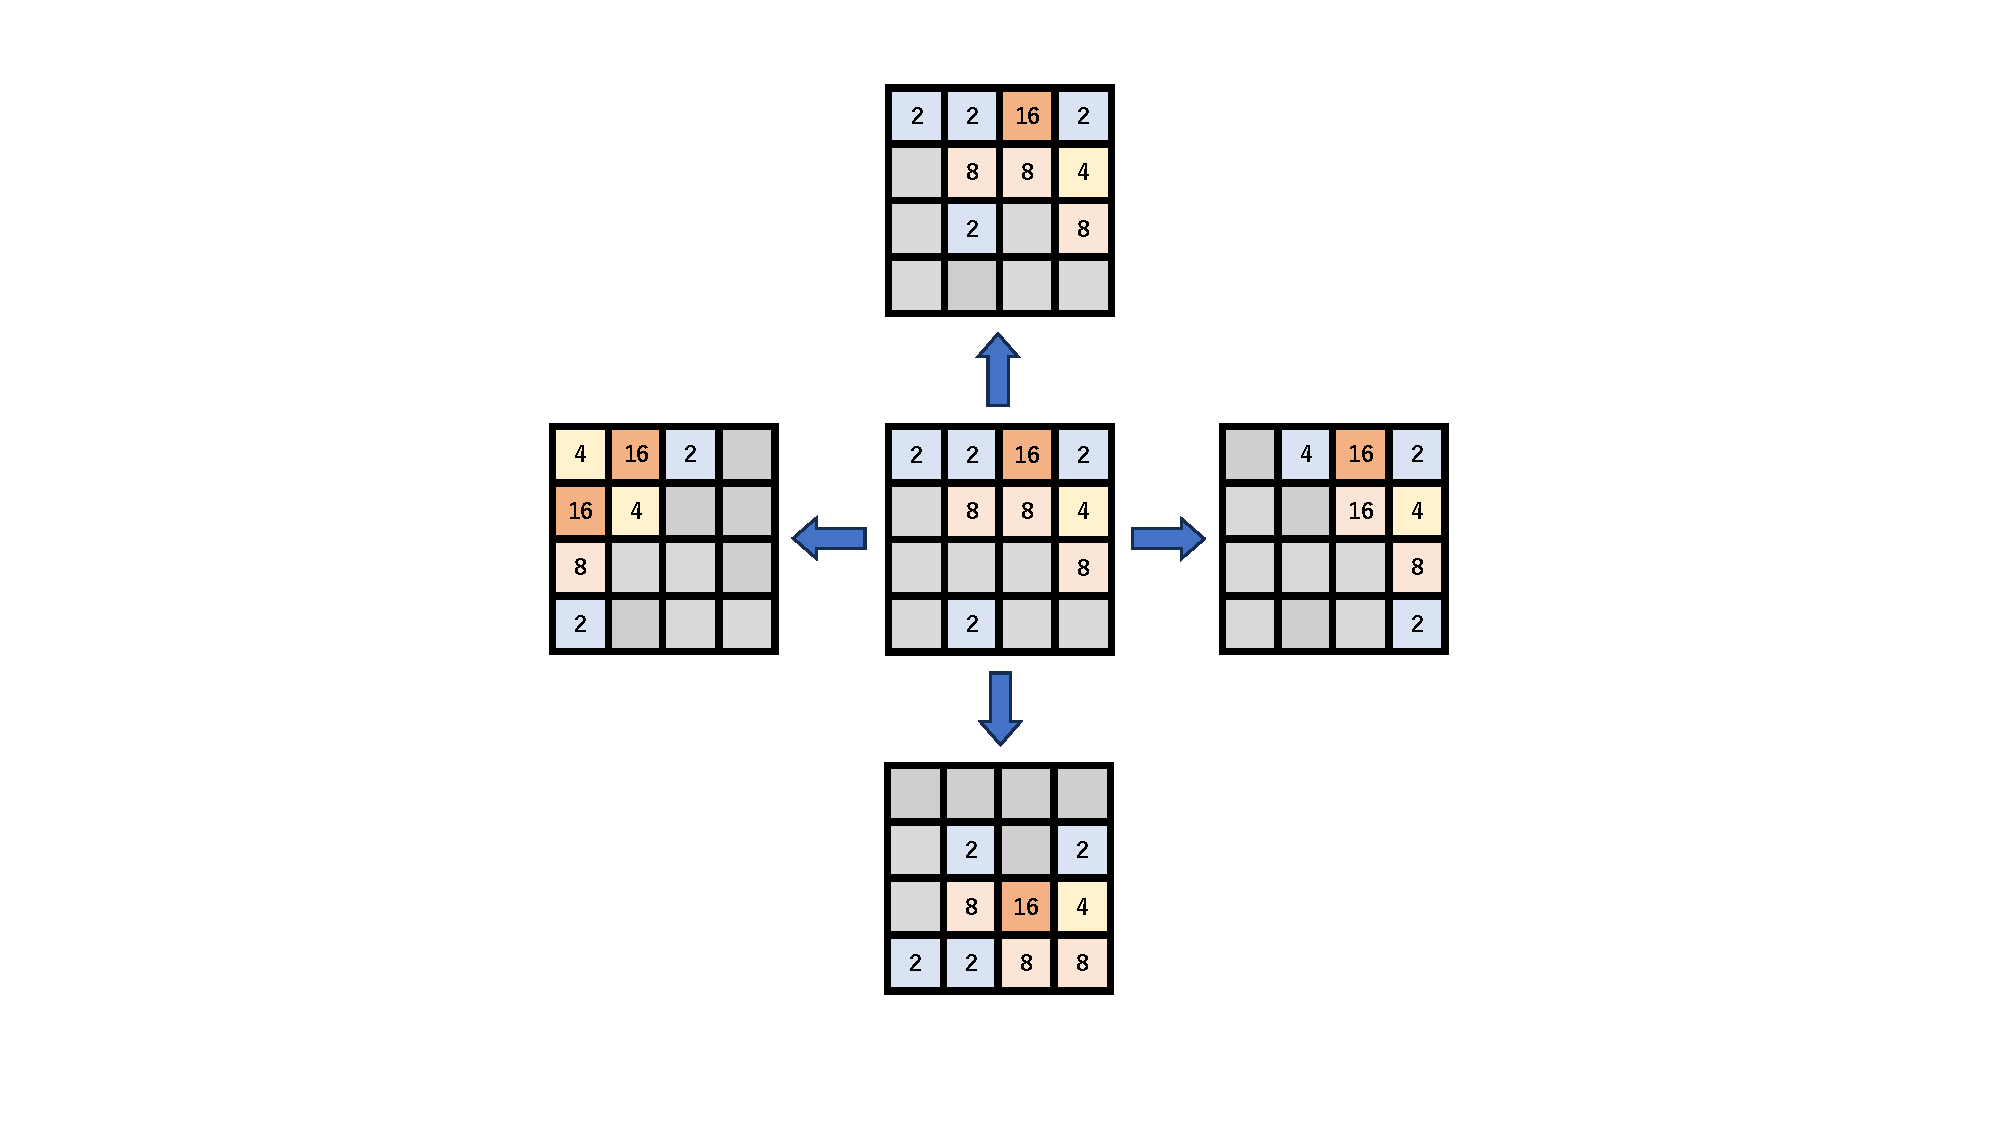
\includegraphics[width=0.8\linewidth{}]{figures/all_directions.pdf}
    \caption{上下左右それぞれへのスライドの例 \label{fig:all_directions}}
\end{figure}

数字タイルのスライド後, 空きマスから等確率に選択されたある1マスに$90\%$の確率で$2$のタイルが, $10\%$の確率で$4$のタイルが置かれる. 
ゲームはプレイヤの行動による数字タイルのスライドと新たな数字タイルの出現を交互に繰り返して進行する.
盤面上の数字タイルが市松模様のようになると, プレイヤが選択可能な行動がなくなったときにゲームは終了する~(図~\ref{fig:terminal}を参照).
\begin{figure}[t]
    \centering
    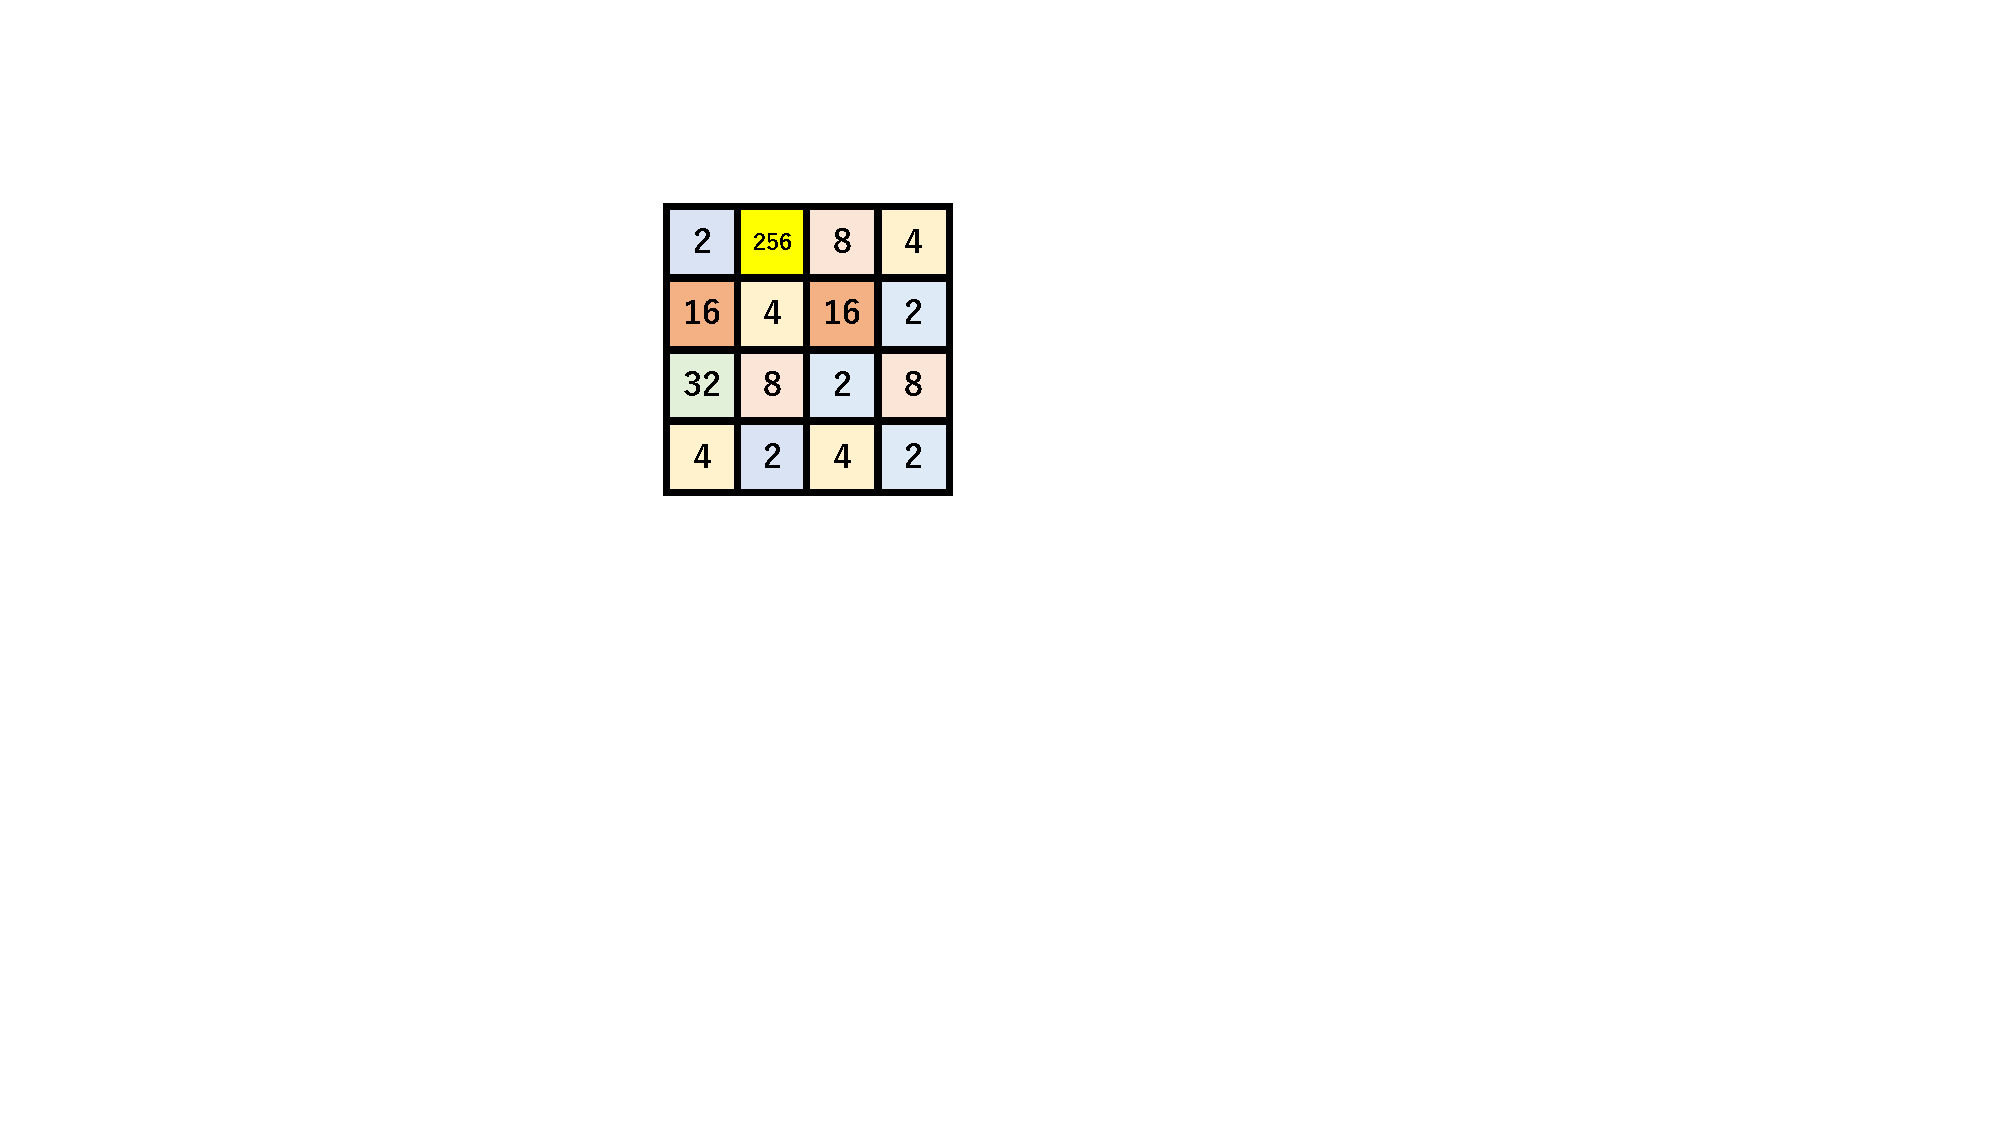
\includegraphics[width=0.2\linewidth{}]{figures/terminal_.pdf}
    \caption{終了状態の例 \label{fig:terminal}}
\end{figure}

ここでプレイヤが行動を選択する盤面を\textgt{状態}, 行動を選択して新たな数字タイルが出現する直前の盤面を\textit{afterstate}と呼ぶ.
図~\ref{fig:transition}に状態$s$からafterstate $s'$を経由して, 次の状態$s_{\text{next}}$に遷移する例を示す.

\begin{figure}[t]
    \centering
    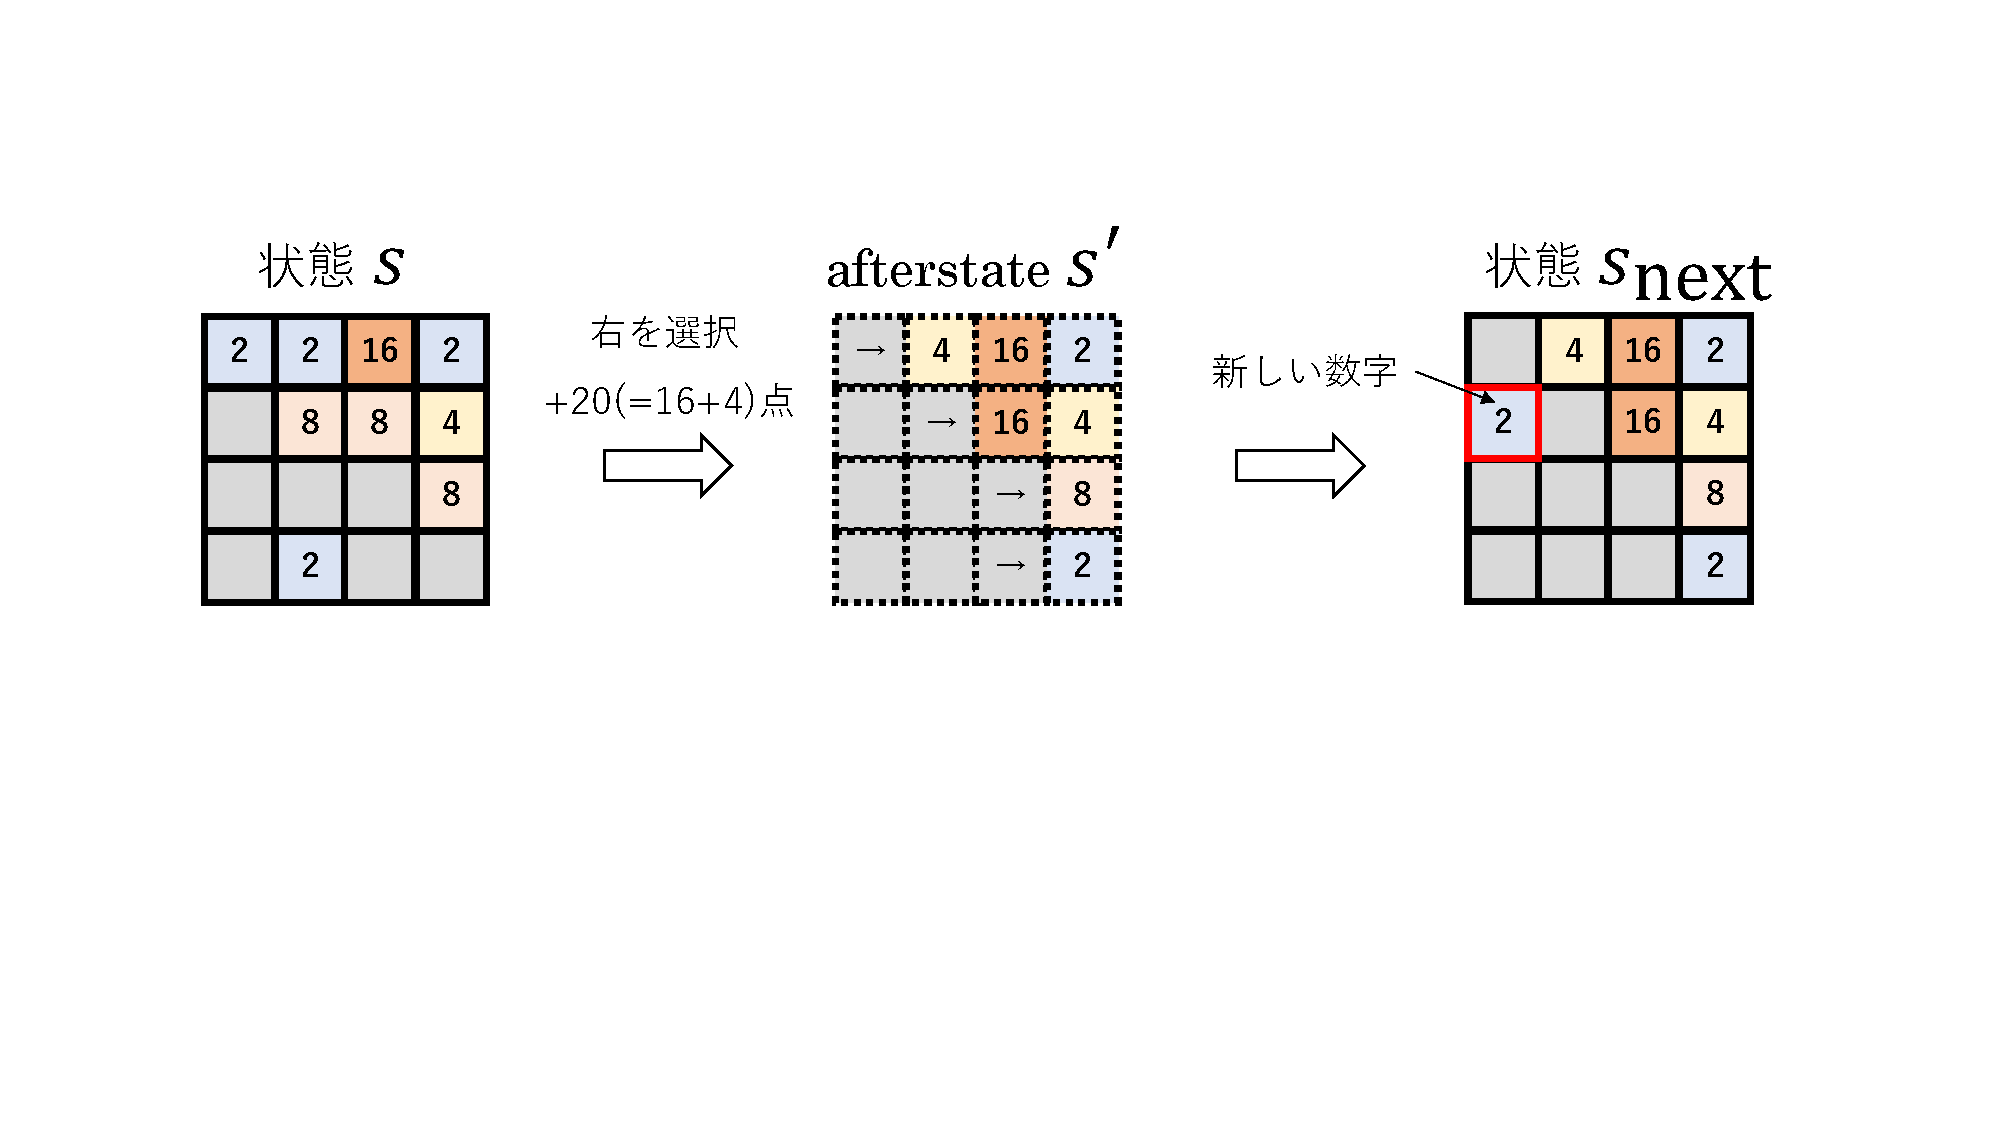
\includegraphics[width=\linewidth{}]{figures/transition_.pdf}
    \caption{状態遷移の例 \label{fig:transition}}
\end{figure}

プレイヤの一般的な目標はゲームのタイトルが示す$2^{11}=2048$のタイルを完成させることだが, それ以降もゲームを続けることができる.

\section{ゲームの進行と時刻}
\label{sec:property}
2048はゲームの性質上, 状態からafterstateへの遷移において盤面上の数字タイルの合計値は不変である~(図~\ref{fig:all_directions}を参照).
盤面上の数字タイルの合計値はafterstateから次の状態への遷移においてのみ変化する.
新しい数字タイルとして$2$か$4$のタイルが出現することで, 数字タイルの合計値はその値の分だけ必ず増加する.
すなわちプレイヤが$1$回行動するたびに, 盤面上の数字タイルの合計値は$2$か$4$ずつ単調に増加する.

よって盤面上の数字タイルの合計値をゲームの進行度合いとして用いることができる.
以降これを\textgt{時刻}と呼ぶ.
例えば図~\ref{fig:transition}では時刻$2\times4+4+8\times3+16=52$の状態$s$が時刻$52+2=54$の状態$s_{\text{next}}$に遷移している.
ゲームの時刻はプレイヤが行動するたびに必ず増加するため, 2048はサイクルの出現しないゲームであることがわかる.



\subsection{ゲームの終了状態}

またゲームの開始盤面をまとめて初期状態と呼ぶことにする.
\chapter{2048と強化学習}
\label{chap:rl}
これまでに2048を対象とした強化学習の研究は数多くなされてきた. 
本章では強化学習の概要, および2048に対する強化学習の先行研究について記述する.

\section{強化学習の概要}
\label{sec:rl_general}
まず本節では2048との関係を踏まえつつ, 一般的な強化学習の概要について記述する.
なお本節の内容は全体に文献~\cite{Sutton1998}を参照して書かれた.

\subsection{マルコフ決定過程}
\label{subsec:mdp}
強化学習は与えられた環境において試行錯誤することを通して, 目標を達成するための戦略や意思決定を学習するための手法である.
学習や意思決定を行う主体はエージェントと呼ばれる.
エージェントは離散タイムステップに従って行動を選択し続け, 環境とやり取りを行う.

このような問題設定はマルコフ決定過程~(MDP)~というモデルによって定式化されている.
MDPは以下の$4$つの要素で構成される. 
\begin{itemize}
  \item 状態集合 $\mathcal{S}$
  \item 行動集合 $\mathcal{A}$
  \item 状態遷移関数$p:\mathcal{S} \times \mathcal{A} \times \mathcal{S} \rightarrow [0,1]$
  \item 報酬関数$r:\mathcal{S} \times \mathcal{A} \times \mathcal{S} \rightarrow \mathbb{R}$
\end{itemize}
エージェントはステップ$t$で状態$S_t \in \mathcal{S}$から行動$A_t \in \mathcal{A}$を選択する.
そして確率$p(S_{t+1}|S_t, A_t)$で次の状態$S_{t+1}$に遷移し, $R_{t+1} = r(S_t, A_t, S_{t+1})$を即時報酬として獲得する.
状態遷移関数と報酬関数は環境のダイナミクスと呼ばれることがある. 
図\ref{fig:mdp}にMDPの概念図を示す.
\begin{figure}[h]
  \centering
  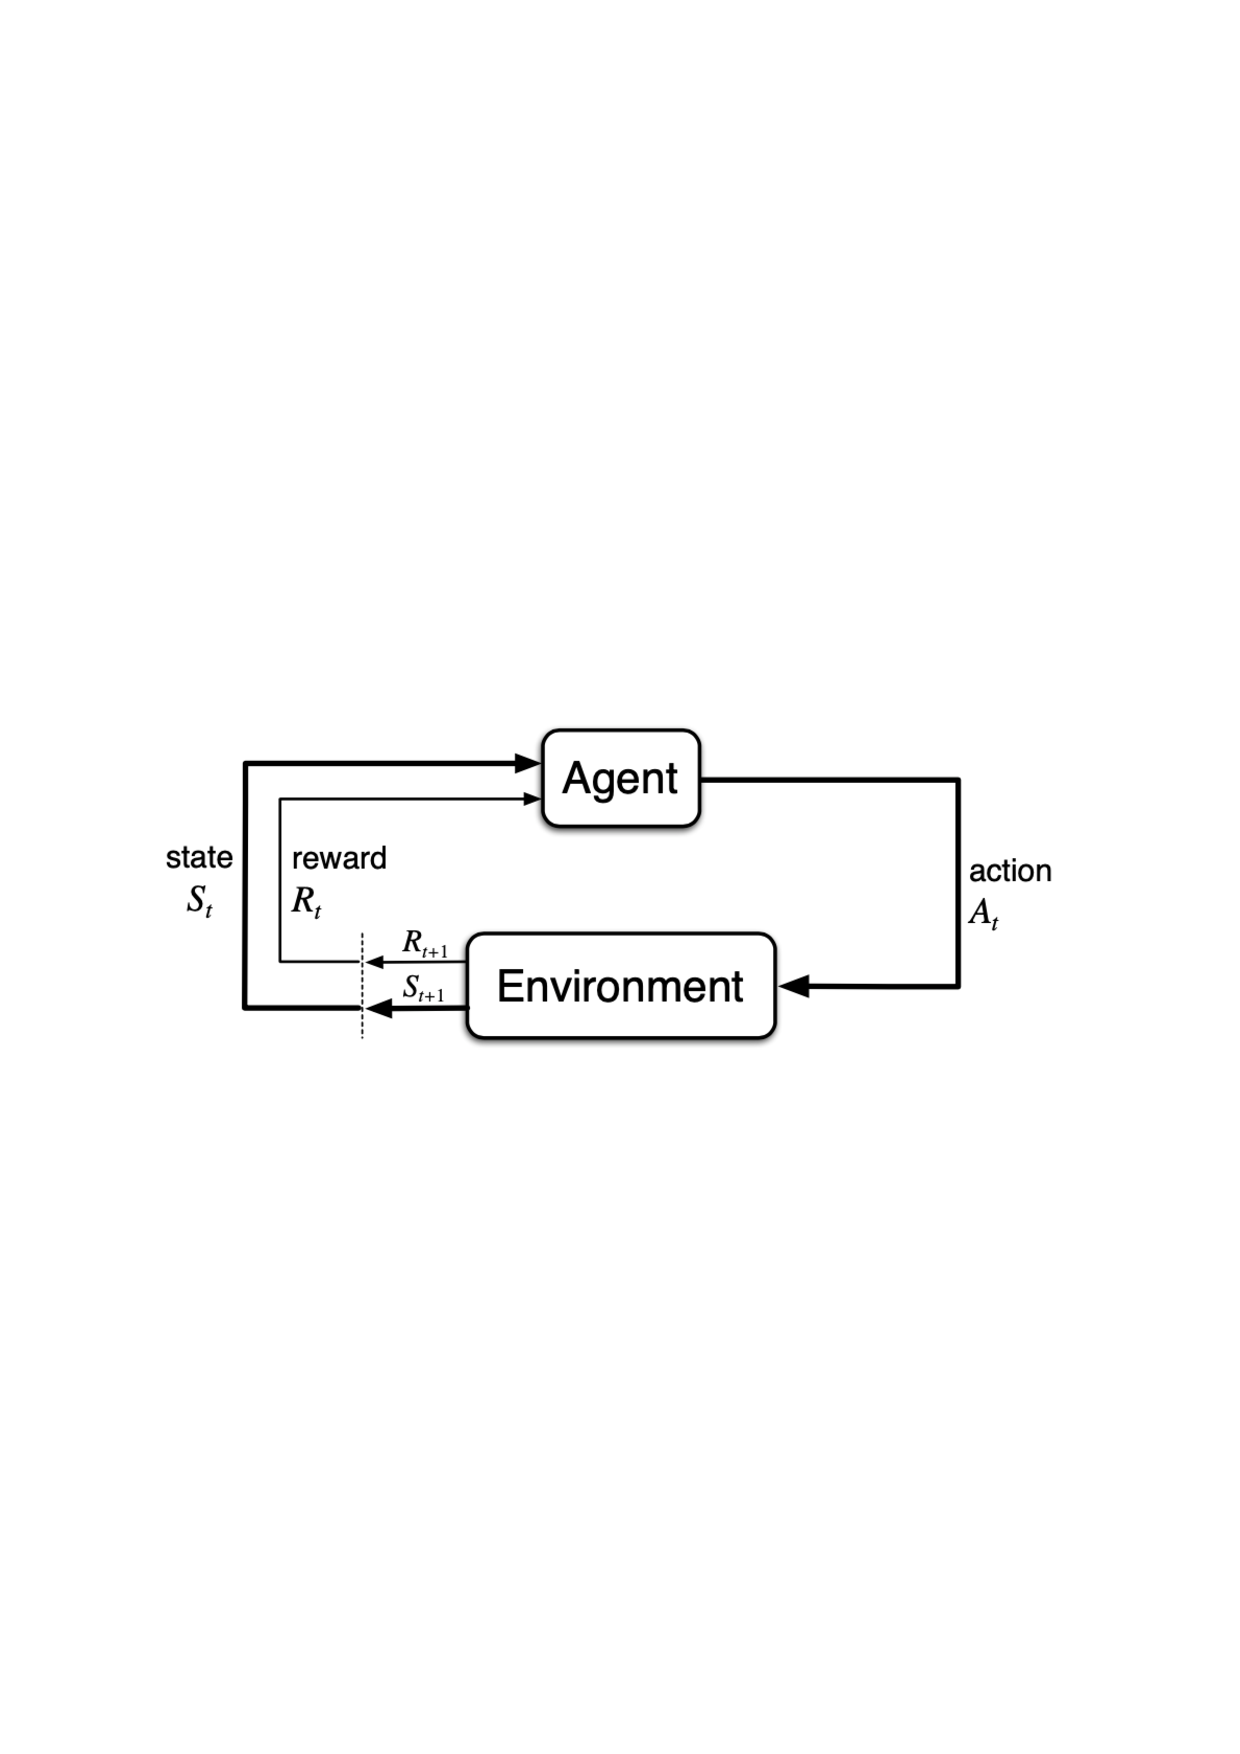
\includegraphics[width=\linewidth{}]{figures/MDP.pdf}
  \caption{MDPの模式図 (文献\cite{Sutton1998}より引用)}
  \label{fig:mdp}
\end{figure}

状態集合と行動集合が有限であるMDPを有限MDPと呼ぶ.
2048は有限MDPにそのまま当てはまるゲームである.
行動集合\textit{A}はプレイが選ぶ上下左右に対応し, 報酬はプレイヤが獲得する得点に直接対応する.

一般に強化学習で扱う問題には, エージェントと環境のやり取りが終わる終了状態が存在するepisodic taskと終了状態が存在しないcontinuing taskが存在する. 
episodic taskではエージェントと環境のやり取りを初期状態から終了状態までのエピソードと呼ばれる単位で分割することができる.
\ref{sec:property}節で説明したように2048は必ず終了するゲームであるため, 以降episodic taskでの定義を確認する. 

\subsection{方策と価値関数}
エージェントがある状態において行動を決定する際の戦略, すなわち確率分布$\pi:S \times A \rightarrow [0,1]$を方策と呼ぶ.
状態価値関数$v_{\pi}(s)$は状態$s$から方策$\pi$に従って行動を選択し続けた場合の累積報酬和の期待値であり, 次のように定義される.
\begin{align}
  v_{\pi}(s) \stackrel{\mathrm{def}}{=} \mathbb{E}_{\pi}\left[\sum_{k=0}^T R_{t+k+1}|S_t=s \right]
\end{align}
同様に状態$s$から行動$a$を選択し, その後方策$\pi$に従って行動を選択し続けた場合の累積報酬和の期待値である行動価値関数$q_{\pi}(s,a)$の定義は以下のようになる.
\begin{align}
  q_{\pi}(s,a) \stackrel{\mathrm{def}}{=} \mathbb{E}_{\pi}\left[\sum_{k=0}^T R_{t+k+1}|S_t=s, A_t=a \right]
\end{align}

強化学習の目標は多くの報酬を獲得できるような良い方策を見つけることである.
価値関数の定義より2つの方策$\pi$と$\pi'$があるとすると, すべての状態$s \in S$について$v_\pi(s) \geq v_{\pi'}(s)$が成り立つならば$\pi$は$\pi'$と等価か$\pi'$よりも良い方策だと言える.
ここで他のすべての方策と比べて等価であるか, それよりも良い方策が少なくとも$1$つ存在する.
これは最適方策$\pi_*$と呼ばれる方策である.
$\pi_*$に従うときの状態価値関数は最適状態価値関数と呼ばれ, $v_*$で表される.
同様に$\pi_*$に従うときの行動価値関数は最適行動価値関数と呼ばれ, $q_*$で表される.
それぞれの具体的な定義を式~\ref{eq:v_opt}, \ref{eq:q_opt}に示す.
\begin{align}
  \label{eq:v_opt}
  v_*(s) &= \max_\pi v_{\pi}(s) \quad \text{for all } s \in S \\
  \label{eq:q_opt}
  q_*(s,a) &= \max_\pi q_{\pi}(s, a) \quad \text{for all } s \in S \text{ and } a \in A(s)
\end{align}
このとき$v_*(s) = \max_{a \in A(s)} q_*(s, a)$であるから, 以下の式が導かれる~(図~\ref{fig:backup}を参照)~.
\begin{align}
  v_*(s) &= \max_{a \in A(s)} q_*(s, a) \\
  \label{eq:bellman_v_opt}
               &= \max_{a \in A(s)} \mathbb{E}[R_{t+1} + v_*(S_{t+1}) | S_t=s, A_t=a] \\
  q_*(s, a) &= \mathbb{E}[R_{t+1} + v_*(S_{t+1}) | S_t=s, A_t=a] \\
  \label{eq:bellman_q_opt}
                  &= \mathbb{E}[R_{t+1} + \max_{a'} q_*(S_{t+1}, a') | S_t=s, A_t=a]
\end{align}
式~\ref{eq:bellman_v_opt}, \ref{eq:bellman_q_opt}はベルマン最適方程式と呼ばれる.
\begin{figure}[h]
  \centering
  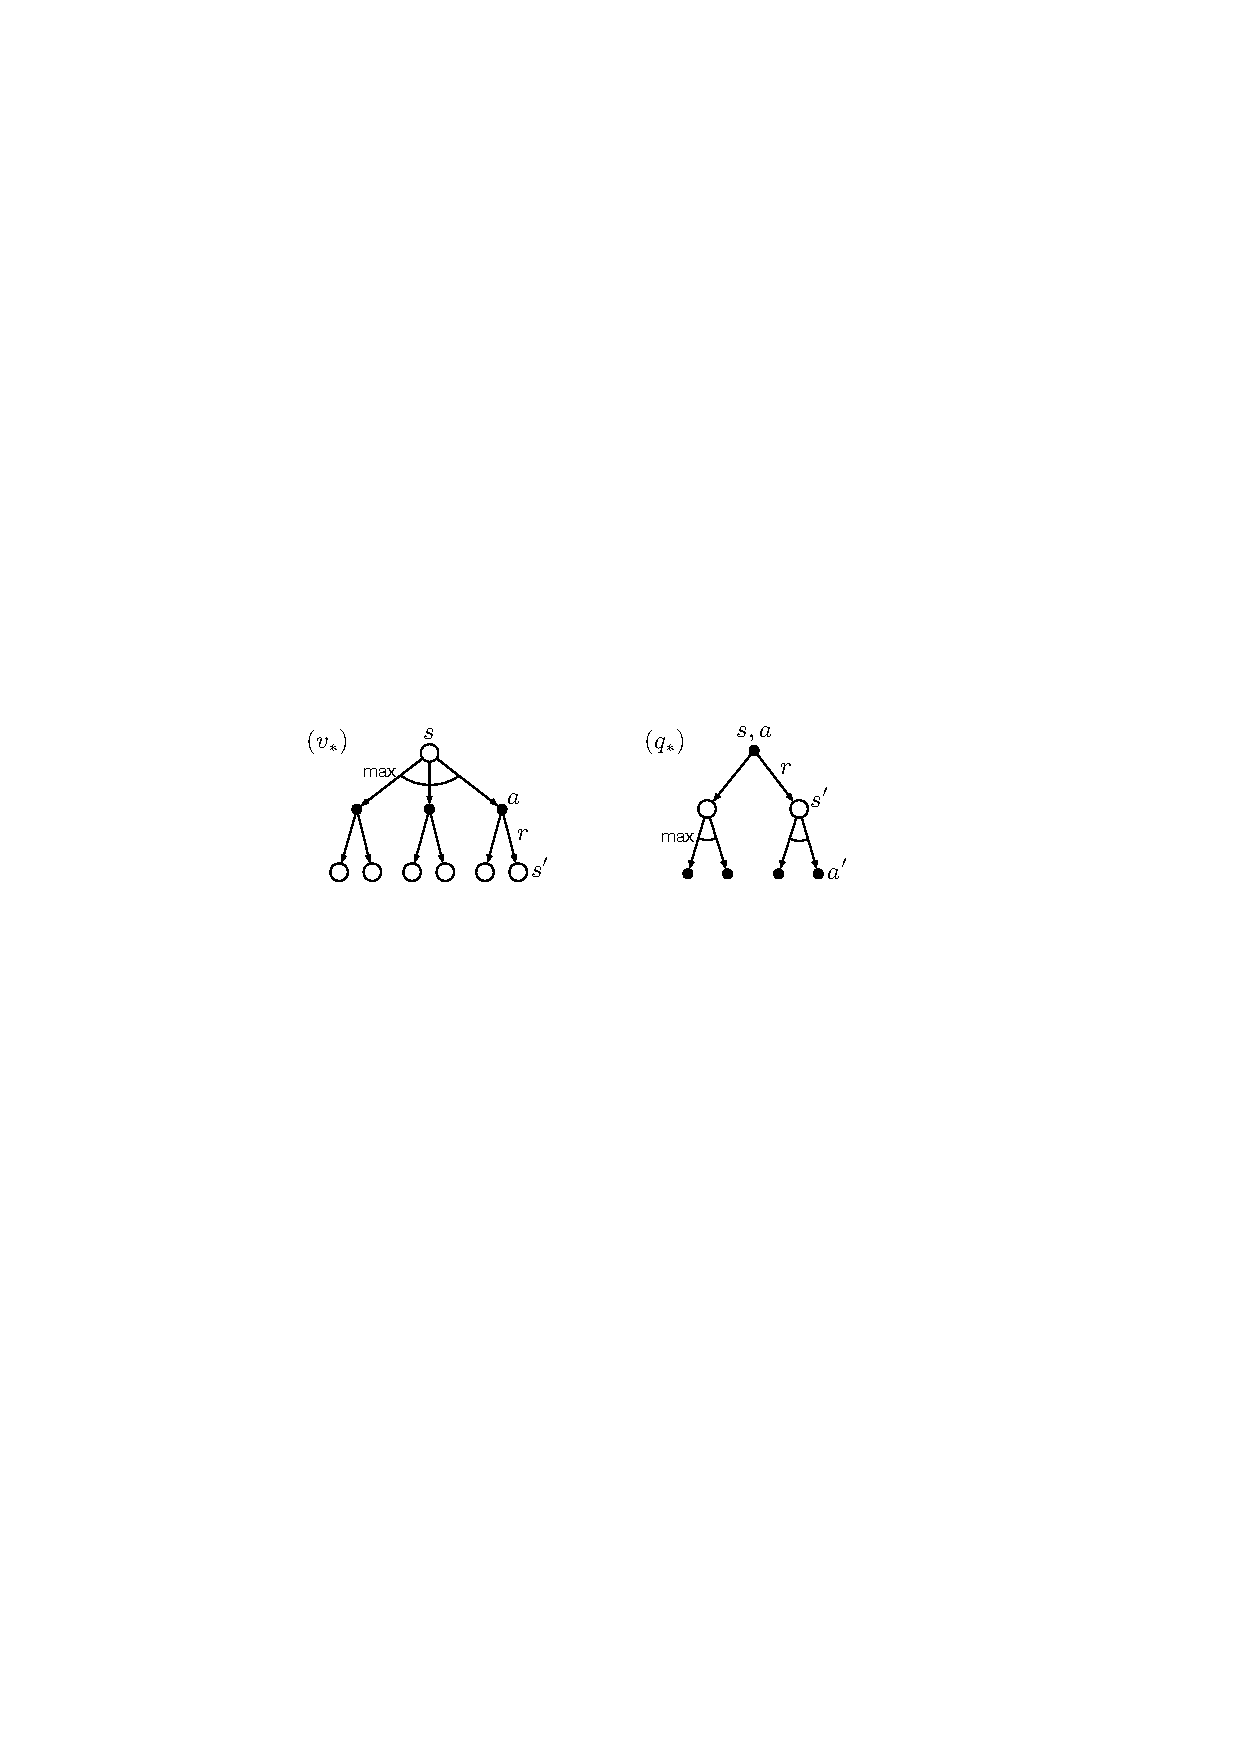
\includegraphics[width=\linewidth{}]{figures/backup.pdf}
  \caption{最適価値関数のバックアップ図 (文献\cite{Sutton1998}より引用)}
  \label{fig:backup}
\end{figure}

\subsection{価値ベースな手法}
状態$s$における最適方策に従った具体的な行動は$\argmax \mathbb{E}[R_{t+1} + v_*(S_{t+1}) | S_t=s, A_t=a]$と, $1$ステップ先の状態を探索してそれらの最適状態価値関数を参照することで計算できる.
最適行動価値関数が参照できれば, $1$ステップ先の状態を探索する必要すらなく, 単に$\argmax q_*(s, a)$を選択すればよい.
最適方策を得るために価値関数を学習する手法は価値ベースな手法と呼ばれる.

Q学習は最も基本的な価値ベースな手法の$1$つで, 最適行動価値関数$q_*$の推定値$Q$を得られた経験から学習する.
状態$S_t$から行動$A_t$を選択し, 報酬$R_{t+1}$を獲得して次の状態$S_{t+1}$に遷移したとする.
このときQ学習は以下の更新式~\ref{eq:q_learning}に従って$Q(S_t, A_t)$を更新する.
\begin{align}
  \label{eq:q_learning}
  Q(S_t, A_t) \leftarrow Q(S_t, A_t) + \alpha [R_{t+1} + \max_a Q(S_{t+1}, a) - Q(S_t, A_t)] 
\end{align}
式~\ref{eq:q_learning}は現在の推定値$Q(S_t, A_t)$を, ベルマン最適方程式~\ref{eq:bellman_q_opt}の右辺の推定値である$R_{t+1} + \max_a Q(S_{t+1}, a)$に近づけていると解釈できる.
任意の$(s, a) \in \mathcal{S} \times \mathcal{A}$について$Q(s,a)$が更新され続けるという条件の下で, Q学習は収束が保証されている.

状態集合や行動集合が大きい場合や有限でない場合には, テーブル形式でQ値を保持することができないため何らかの関数近似を行う必要がある.
近年では深層学習~\cite{DeepLearning}の研究の発展により, 関数近似の方法としてニューラルネットワークが用いられることが多い.
価値関数や方策をニューラルネットワークで近似する手法は, まとめて深層強化学習と呼ばれる.

Q値をニューラルネットワークで近似する, Deep Q Network~(DQN)~\cite{DQN}は深層強化学習の先駆けとして有名な手法である. 
DQNはエージェントが蓄積したデータからバッチサイズ個をランダムにサンプルし, これらをニューラルネットワークの学習に使用するExperience Replayを提案した.
Experience Replayによって学習データは適度にばらつき, ニューラルネットワークの学習は安定化する.
Schaulらが提案したPrioritized Experience Replay~\cite{prioritized}は一様ランダムではなく, priorityという重みに従ってデータをサンプルするExperience Replayである.
優先的に学習したいデータを積極的に訓練に用いることで, 学習効率が上がることが期待される.
価値ベースな深層強化学習手法はDQNの発表以降, 様々な工夫が提案され続けている.
詳細は文献~\cite{deepRL}の$4$節などを参照されたい.

\subsection{方策ベースな手法}
方策を直接パラメタライズされた関数で近似し, パラメータを学習する手法を全般に方策ベースな手法と呼ぶ.
なお方策ベースな手法においても価値関数の学習を行うことはあるが, 良い方策のパラメータを学習するために必要とするものであり, 直接的な行動の選択には関与しない.

方策のパラメータ$\pmb{\theta}$は目的関数$J(\pmb{\theta})$を最大化するように更新される.
$J(\pmb{\theta})$は, 方策$\pi_{\pmb{\theta}}$に従ったときの初期状態$s_0$の価値$v_{\pi_{\pmb{\theta}}}(s_0)$と定義することができる.
このとき方策$\pi$のもとで状態$s$を訪れる確率を$\mu(s)$とすると, $\nabla J(\pmb{\theta})$は以下の方策勾配定理によって求めることができる.
\begin{align}
  \label{eq: policy_gradient_theorem}
  \nabla J(\pmb{\theta}) \propto \sum_s \mu(s) \sum_a q_{\pi}(s,a) \nabla \pi(a|s, \pmb{\theta})
\end{align}
さらに以下のように変形する.
\begin{align}
  \nabla J(\pmb{\theta}) &\propto \sum_s \mu(s) \sum_a q_{\pi}(s,a) \nabla \pi(a|s, \pmb{\theta}) \notag \\
  & = \mathbb{E}_{\pi} \left[\sum_a q_\pi(S_t, a) \nabla \pi(a|S_t, \pmb{\theta})\right] \notag \\
  & = \mathbb{E}_{\pi} \left[\sum_a \pi(a|S_t, \pmb{\theta}) q_\pi(S_t, a) \frac{\nabla \pi(a|S_t, \pmb{\theta})}{\pi(a|S_t, \pmb{\theta})}\right] \notag \\
  & = \mathbb{E}_{\pi} \left[q_\pi(S_t,A_t) \frac{\nabla \pi(A_t|S_t, \pmb{\theta})}{\pi(A_t|S_t,\pmb{\theta})}\right] \notag \\
  & = \mathbb{E}_{\pi} \left[q_\pi(S_t,A_t) \nabla \ln \pi(A_t|S_t, \pmb{\theta}) \right] \notag \\
\end{align}
よって学習率を$\alpha$とすると, パラメータ$\pmb{\theta}$の更新式が導かれる.
\begin{align}
  \label{eq:reinforce}
  \pmb{\theta}_{t+1} \leftarrow \pmb{\theta}_{t} + \alpha \left[q_\pi(S_t,A_t) \nabla \ln \pi(A_t|S_t, \pmb{\theta}) \right]
\end{align}
ただし未知の値$q_\pi(S_t,A_t)$を, 学習データから推定する必要がある.
Williams~\cite{Williams:92}は$q_\pi(S_t,A_t)$の推定値として, $S_t$から$A_t$を選択して実際に獲得した報酬の総和$G_t = \Sigma_{k=0}^{T} R_{t+k+1}$を用いることを提案した.
$G_t$は$q_\pi(S_t,A_t)$の不偏推定量としての性質をみたす一方で, 分散が大きく学習が安定しない.
またパラメータの更新をエピソードが終了するまで行うことができない.

ここで式~\ref{eq: policy_gradient_theorem}において, 行動$a$に依存しない定数を$b(s)$として$\Sigma_a b(s) \nabla \pi(a|s,\pmb{\theta}) = b(s) \nabla \Sigma_a \pi(a|s, \pmb{\theta}) = 0$に注目すると, 以下の式~\ref{eq:reinforce_baseline}が成り立つ.
\begin{align}
  \label{eq:reinforce_baseline}
  \nabla J(\pmb{\theta}) \propto \sum_s \mu(s) \sum_a \left(q_{\pi}(s,a) - b(s)\right) \nabla \pi(a|s, \pmb{\theta})
\end{align}
$b(s)$として$s$の価値関数$v_{\pi}(s)$を考えることが一般的である.
$q_{\pi}(s,a) - v_{\pi}(s)$は, 状態$s$で行動$a$をとることが他の行動をとることに比べて, どれくらい良いかを示す値で一般的にアドバンテージと呼ばれる.
よってパラメータ更新式~\ref{eq:reinforce}中の$q_\pi(S_t,A_t)$の代わりに, アドバンテージ$q_\pi(S_t,A_t) - v(S_t)$を推定する.
そのために方策関数の学習と同時に, 価値関数$v_\pi$の推定値$V$を学習する.
$q_\pi(S_t,A_t) = \Sigma_{k=0}^{n-1} R_{t+k+1} + v_\pi(S_{t+n})$であるから, 以下の方策パラメータ$\pmb{\theta}$の更新式~\ref{eq:actor_critic}が導かれる.
\begin{align}
  \label{eq:actor_critic}
  \pmb{\theta}_{t+1} \leftarrow \pmb{\theta}_{t} + \alpha \left[\sum_{k=0}^{n-1} \big(R_{t+k+1} + V(S_{t+n}) - V(S_{t+n})\big) \nabla \ln \pi(A_t|S_t, \pmb{\theta}) \right]
\end{align}
ここで$\Sigma_{k=0}^{n-1} R_{t+k+1} + v_\pi(S_{t+n})$は$n$ステップリターンと呼ばれる.
$n$をエピソードの終了時刻$T$とすると, $n$ステップリターンは$G_t$に一致する.
このように学習した価値関数を行動の良さを評価するために用いる手法は, 全般にactor-criticな手法と呼ばれる.

Mnihら~\cite{A3C}が提案したasynchronous advantage actor-critic~(A3C)~は, 方策関数と価値関数をニューラルネットワークにより近似したactor-criticな手法で, Atariや物理シミュレーションの実験で高い成果を収めた.
A3Cの発表以降, 方策ベースな深層強化学習の研究は数多くなされている.
特にSchulmanらが提案したProximal Policy Optimization~(PPO)~\cite{PPO}は有名手法の$1$つである.

\subsection{AlphaZeroとMuZero}
\label{subsec:zero}
Silverらが提案したAlphaZero~\cite{AlphaZero}は, 囲碁やチェスなどの二人零和完全確定情報ゲームを対象とした有力な深層強化学習手法である.
AlphaZeroは盤面の特徴量を入力として, その盤面における方策と価値を出力するニューラルネットワークを持つ.
これをモンテカルロ木探索~(MCTS)~による自己対戦を通して得たデータから学習する.
そのため人間の棋譜などの教師データを使うことなく, 囲碁, 将棋, チェスにおいて当時の有力なプログラムを上回る強さを示して注目を集めた.

AlphaZeroはMCTSを行うにあたって, ゲームのルールや環境のダイナミクスが既知であることを前提としている.
すなわち現在の状態$s_t$から行動$a_t$を選択した後の状態$s_{t+1}$を, $s_t$のみ観測している状況から知ることができる必要がある.
そのためAlphaZeroは複雑なダイナミクスを持つAtariなどのゲームには適用することが難しい.
Schrittwieserらが提案したMuZero~\cite{MuZero}は, ニューラルネットワークで環境のダイナミクスをモデル化し, 学習することを提案した.
MuZeroは二人零和完全確定情報ゲームにおいてAlphaZeroと同等の強さ, Atariにおいて当時の有力手法と同等以上の性能を示した.
\ref{subsec: stochastic_muzero}節でMuZeroを確率的な環境に対応できるように拡張した, Stochastic MuZeroについて述べる.
そこでMCTSの具体的な方法や, ニューラルネットワークの学習方法について述べる.

\section{2048への強化学習の応用}
\label{sec:rlto2048}
\ref{sec:rl_general}節では強化学習一般の概要について説明した.
これを踏まえて本節では, 2048を対象とした強化学習研究の先行研究について概説する.

\subsection{TD afterstate学習}
\label{subsec: td_afterstate}
Szubertら~\cite{Szubert}はTD afterstate学習と呼ばれる価値ベースの強化学習手法を提案した.
2048はゲームの性質上, 状態$s$から行動$a$をとって獲得する得点$r(s,a)$と遷移するafterstate $s'$は決定的である.
よってafterstate $s'$の最適価値を$v_*'(s')$と表すと, 行動価値$q_*(s,a)$は$q_*(s,a) = r(s,a) + v_*'(s')$と分解できる.
そこでTD afterstate学習は, Q値ではなくafterstateの価値$v_*'$の推定値$V'$を式~\ref{eq:td_afterstate}に従って更新する.
\begin{align}
  \label{eq:td_afterstate}
  V'(S_{t}^{'}) \leftarrow  V'(S_{t}^{'}) + \alpha [R_{t+1} + V'(S_{t+1}^{'}) - V'(S_{t}^{'})]
\end{align}
式~\ref{eq:td_afterstate}はQ学習の更新式~\ref{eq:q_learning}において, $Q(S_t, A_t) = R(S_t, A_t) + V'(S_{t}^{'})$として書き直したものと見ることができる.

SzubertらはN-tupleネットワークというヒューリスティックな盤面評価関数を用いて$V'$を表現し, $2048$のタイルを$98$\%の確率で到達させることに成功した.
Jaskowski~\cite{DBLP:journals/corr/Jaskowski16}はこれに様々な工夫を加えた学習方法を提案し, 最終的にexpectimax探索を$1$手$1$秒の制限で行うことで平均$609,104$点を獲得するプレイヤを開発した.
松崎~\cite{KiminoriMatsuzaki2021}はニューラルネットワークによって表現した$V'$を学習させ, $3$-ply expectimax探索を行うことで平均$406,927$点を達成した.

Szubertらは文献~\cite{Szubert}でN-tupleネットワークを用いたQ学習の実験も行ったが, TD afterstate学習の性能を大きく下回る結果になったことを報告している.
TD afterstate学習は観測している状態$s$からafterstate $s'$への遷移までをシミュレートする, いわば$0.5$手読みの探索を行っているため, $0$手読みのQ学習と比べて学習しやすいと考えられる.

\subsection{Afterstate PPO}
\ref{subsec: td_afterstate}節では, 価値ベースな手法であるTD afterstate学習が2048において主流な強化学習手法の$1$つであることを説明した.
一方で, 2048において目立った方策ベースな強化学習手法は
山下ら~\cite{afterstate_ppo}はPPO~\cite{PPO}を2048に工夫して適用する, Afterstate PPOという手法を提案した.
すなわち状態$s$から行動$a$をとったときのafterstateをニューラルネットワークの入力とし, その出力を行動$a$の選択確率のロジットとする.
通常のPPOでは全く学習が進まなかった一方で, Afterstate PPOは学習後2048のタイルを平均約$50\%$の割合で完成させることに成功した.

\subsection{Stochastic MuZero}
\label{subsec: stochastic_muzero}
Antonoglouらが提案したStochastic MuZero~\cite{StochasticMuZero}は~\ref{subsec:zero}節で述べたMuZeroを, 確率的な環境にも対応できるように拡張した手法である.
Stochastic MuZeroは確率的ゲームである2048とバックギャモンでMuZeroを大きく上回るパフォーマンスを発揮した.
さらにランダム性のない囲碁においてもMuZeroと同等のレーティングを達成し, 対象とするドメインが幅広いことを示した.
2048においては, \ref{subsec: td_afterstate}節で述べたTD afterstate学習の先行研究~\cite{DBLP:journals/corr/Jaskowski16}と比較して, 一切のドメイン知識を必要とせず, より優れたパフォーマンスを出したことが強調された.
一方で, 論文内で示されたStochastic MuZeroの最終的な平均スコアは約$50$万点で, expectimax探索を行うことで平均$609,104$点を達成した文献~\cite{DBLP:journals/corr/Jaskowski16}の結果を明確に上回るとはいえない.

Stochastic MuZeroは方策・価値ニューラルネットワークに加えて, 環境のダイナミクスモデルをニューラルネットワークにより推論する.
これらのニューラルネットワークを, モンテカルロ木探索~(MCTS)~によるプランニングを行って得た学習データを用いて訓練する.
以下ではAlphaZeroのように, 環境のダイナミクスを既知とした場合におけるStochastic MuZeroの方法を, 2048に適用することを想定して具体的に説明する.
説明の便宜上これを本稿では, 2048-AlphaZeroと呼ぶことにする.
Stochastic MuZeroの環境のダイナミクスモデルの学習方法については, 文献~\cite{StochasticMuZero}の$4$節を参照されたい.

\subsubsection{2048-AlphaZeroのMCTS}
\label{subsubsec:mcts}
2048-AlphaZeroは$2$つのニューラルネットワークを持つ.
$1$つ目は, 状態盤面$s$の特徴量を入力として$s$における方策, $s$の価値を出力するニューラルネットワーク$f$である.
$2$つ目は, afterstate盤面$s'$の特徴量を入力として$s'$の価値を出力するニューラルネットワーク$g$である.
$2$つのニューラルネットワーク$f$と$g$を用いてMCTSを実行する.

\ref{sec:rule}節で述べたように, 2048は状態とafterstateという$2$種類の盤面が交互に繰り返される.
そのため2048-AlphaZeroはMCTSにおいて, それぞれに対応する状態ノードとafterstateノードという$2$種類のノードから成る探索木を用いる~(文献~\cite{StochasticMuZero}ではそれぞれdecisionノード, chanceノードと呼ばれた).
探索木中のそれぞれのノード$s$は, 以下の$5$つの統計量を管理する.
\begin{itemize}
  \item $N(s) \cdots$探索中に$s$を訪問した回数
  \item $W(s) \cdots$ $s$を根とする部分木中のノードの価値の推定値の合計
  \item $Q(s) \cdots$ $s$を根とする部分木中のノードの価値の推定値の平均~($W(s) / N(s)$)
  \item $P(s) \cdots$ $s$の親から$s$への遷移確率
  \item $R(s) \cdots$ $s$の親から$s$へ遷移するときに獲得する即時報酬~(得点)
\end{itemize}
MCTSは選択, 評価, 逆伝播, 展開の$4$つのステップを繰り返すことで, 探索木を大きくする.
この$4$つのステップはまとめてシミュレーションと呼ばれる.
すなわちシミュレーションを繰り返すことで深い探索を行い, 良い行動を選択することができる.
以下ではそれぞれのステップについて説明する.

\paragraph{選択}
現在のゲーム木の根ノード$s_0$~(decisionノード)~から有望な子ノードを選択し, これを葉ノード$s_L$に至るまで辿り続ける.
decisionノード$s_d$においては, 以下のPUCT式~\ref{eq:puct}が最大となるような子chanceノード$s_c$を選択する.
\begin{align}
  Q(s_c) + C(s_c)P(s_c)\frac{\sqrt{1+N(s_d)}}{1+N(s_c)}
  \label{eq:puct}
\end{align}
ただし$C(s_c)$は探索率を表す.
これは現段階での価値の推定値$Q(s_c)$と探索項$C(s_c)P(s_c)\sqrt{1+N(s_d)}/(1 + N(s_c))$を合計したものである.
$N(s_c)$が小さい子ノードほど探索項は大きな値を示す.
一方chanceノード$s_c$においては, 単にそれぞれの子decisionノード$s_d$への遷移確率$P(s_d)$に従って確率的に選択する.

\paragraph{評価~(図~\ref{fig:evaluate})}
選択のステップの葉ノード$s_L$をニューラルネットワークにより評価する.
$s_L$がdecisionノードである場合には, $s_L$における方策$\pi(\cdot|s_L)$および$s_L$の価値を$v_L$を得る.
$s_L$がchanceノードである場合には, $s_L$の価値$v_L$のみを得る.

\paragraph{展開~(図~\ref{fig:expand})}
$s_L$がdecisionノードである場合には, $s_L$に対応する状態から遷移可能なafterstateを$s_L$の子chanceノードとして探索木に追加する.
それぞれの子chanceノード$s_c$について, $P(s_c) = \pi(s_c|s_L)$とする.

$s_L$がchanceノードである場合には, $s_L$に対応するafterstateから遷移可能な状態を$s_L$の子decisionノードとして探索木に追加する.
それぞれの子decisionノード$s_d$について, $P(s_d)$は$s_L$に対応するafterstateから$s_d$に対応する状態へ遷移する環境の確率とする.

\paragraph{逆伝播~(図~\ref{fig:backpropagate})}
$s_L$について, $N(s_L, a)=0, W(s_L, a)=0, Q(s_L, a)=0$と初期化する.
さらに
さらに$s_0$から$s_L$に至る各ノード$s$について, 以下のように各統計量の値を更新する.
\begin{align*}
  N(s) &\leftarrow N(s) + 1 \\
  W(s) &\leftarrow W(s) + v_L \\
  Q(s) &\leftarrow \frac{W(s)}{N(s)}
\end{align*}

\begin{figure}
  \begin{subfigure}[T]{0.4\columnwidth}
    \centering
    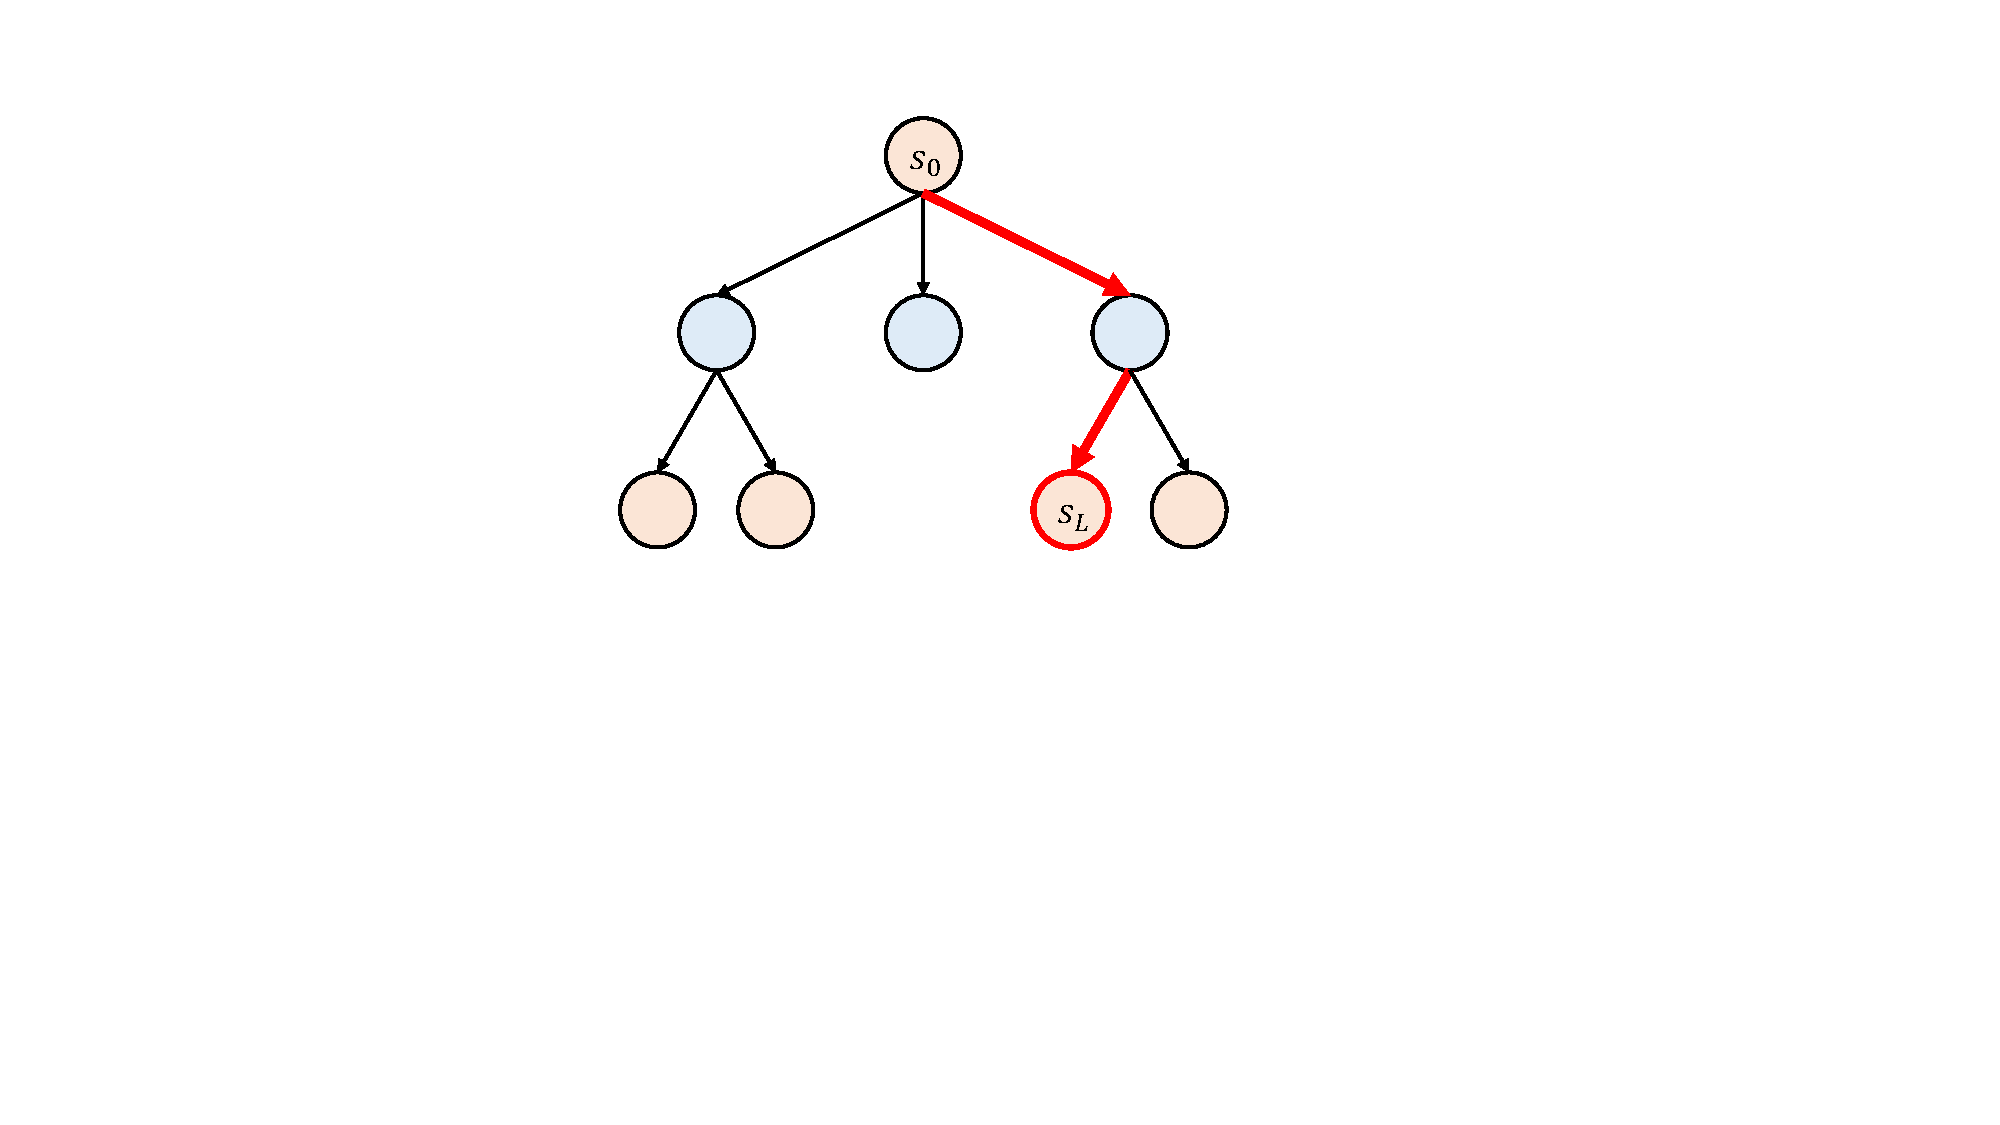
\includegraphics[width=\columnwidth]{figures/selection_.pdf}
    \caption{選択}
    \label{fig:selection}
  \end{subfigure}
  \begin{subfigure}[T]{0.4\columnwidth}
    \centering
    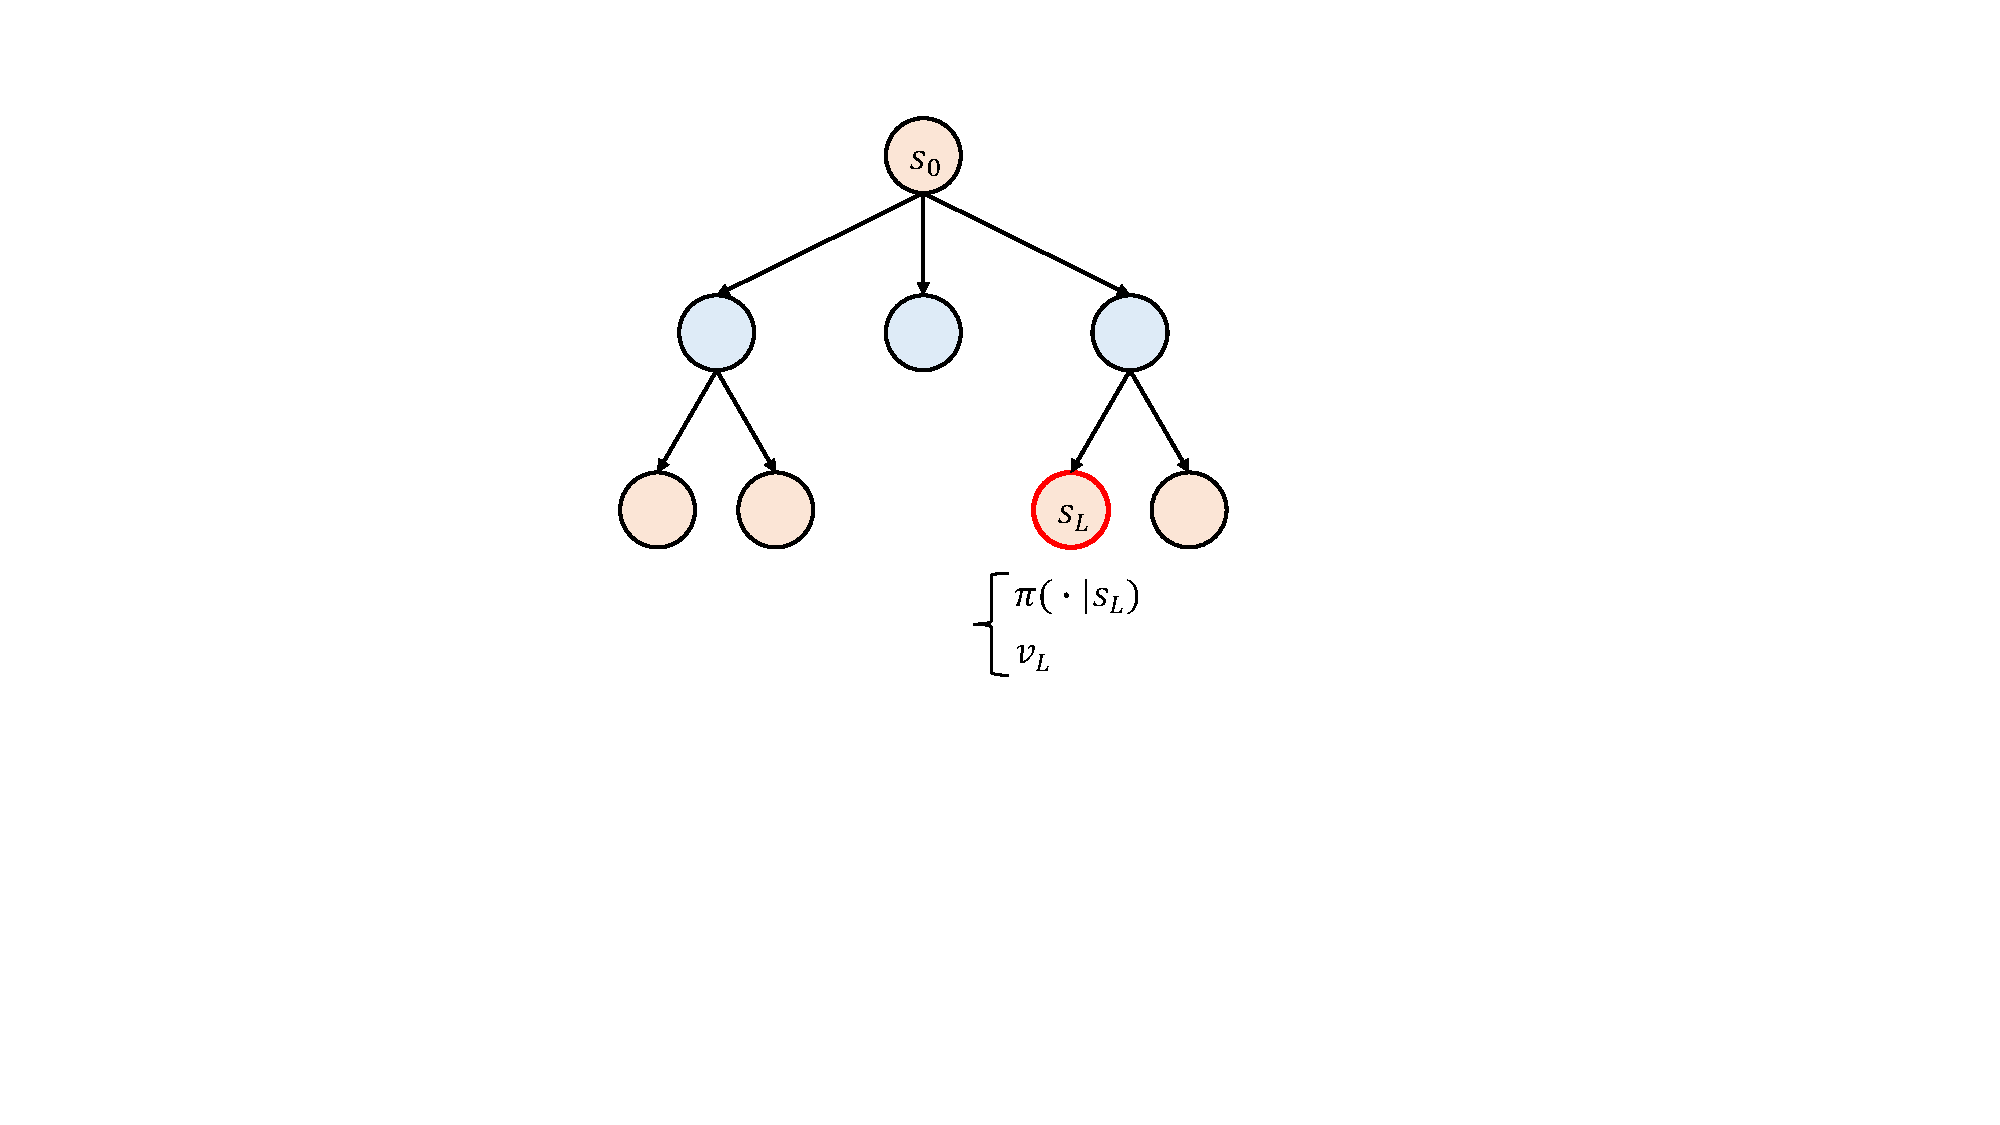
\includegraphics[width=\columnwidth]{figures/evaluate_.pdf}
    \caption{評価}
    \label{fig:evaluate}
  \end{subfigure}
  \begin{subfigure}[T]{0.4\columnwidth}
    \centering
    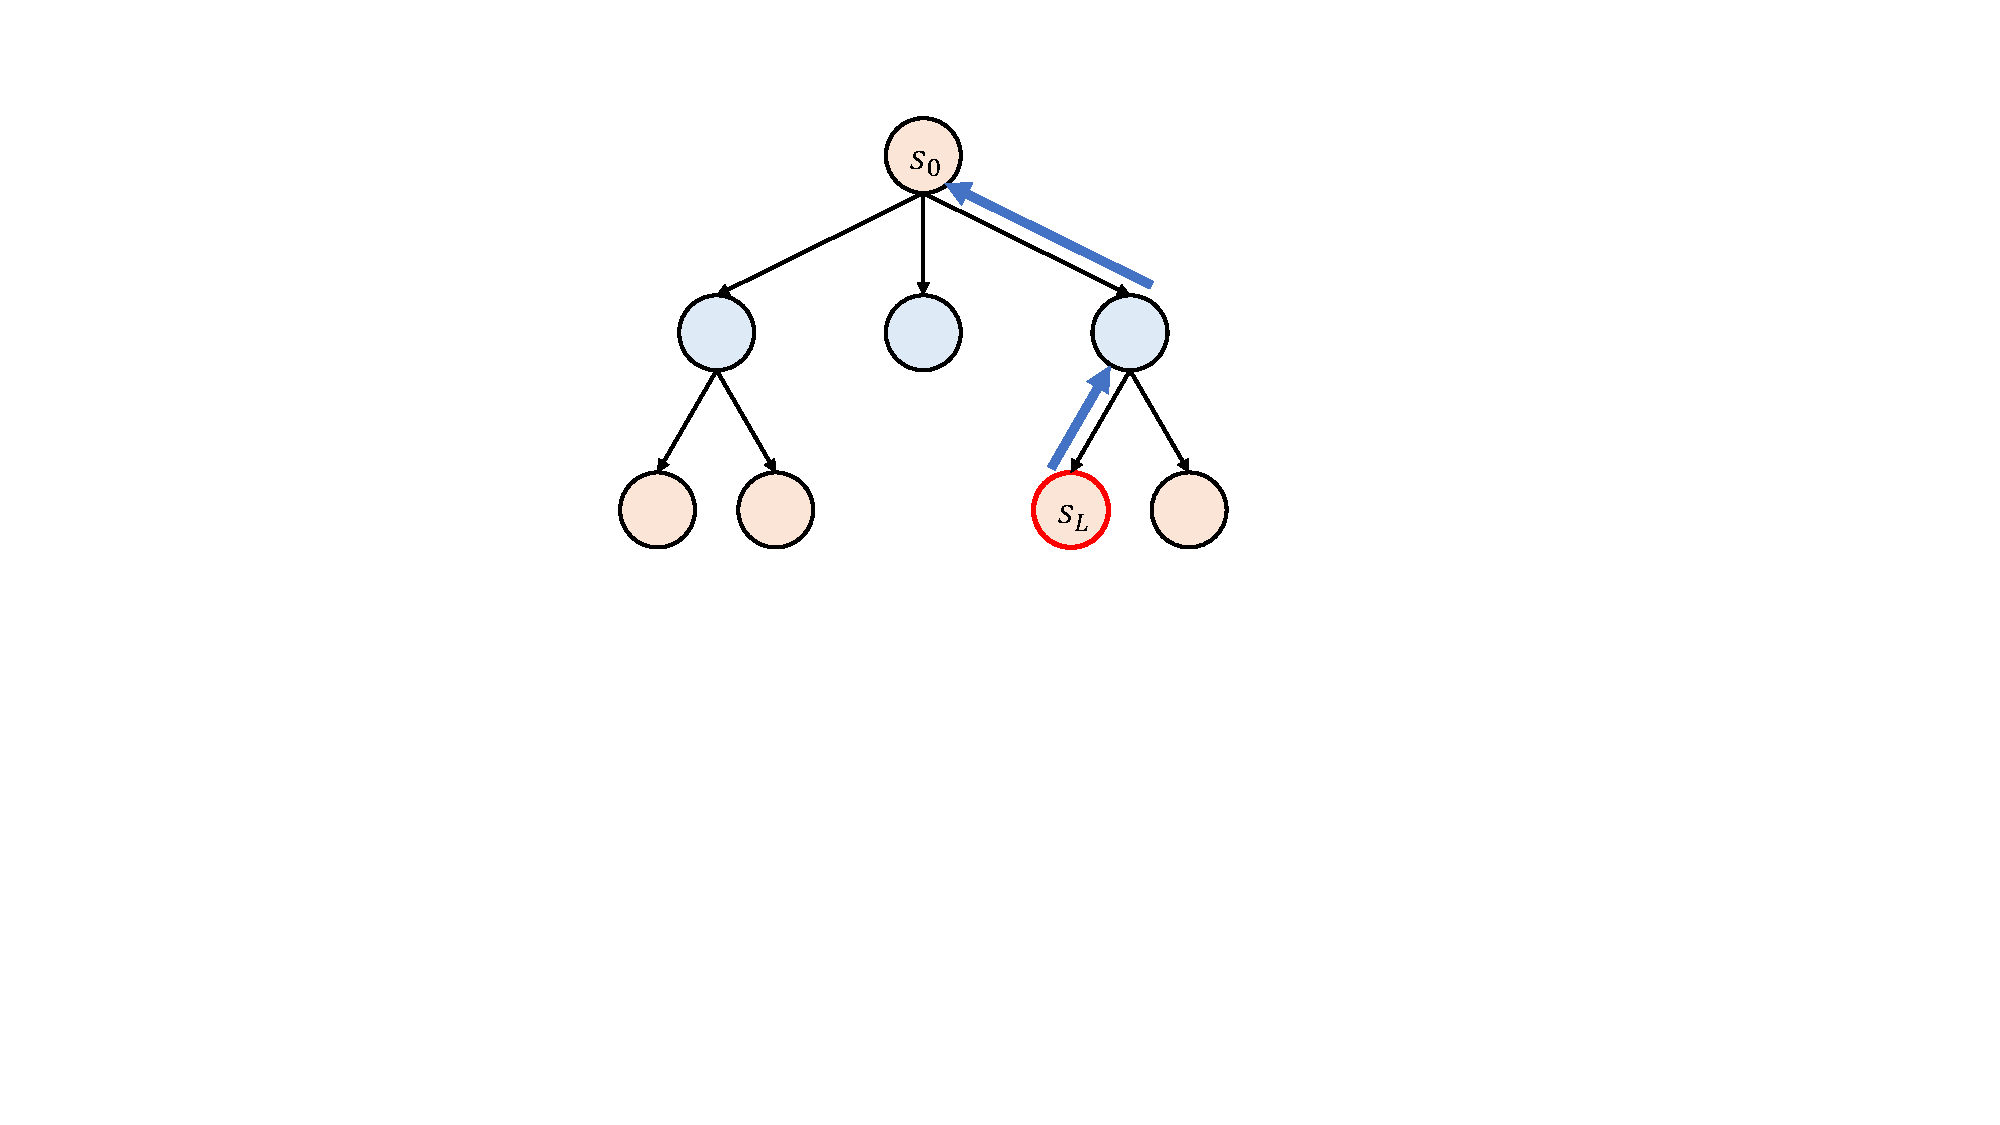
\includegraphics[width=\columnwidth]{figures/backpropagate_.pdf}
    \caption{逆伝播}
    \label{fig:backpropagate}
  \end{subfigure}
  \hspace{3cm}
  \begin{subfigure}[T]{0.4\columnwidth}
    \centering
    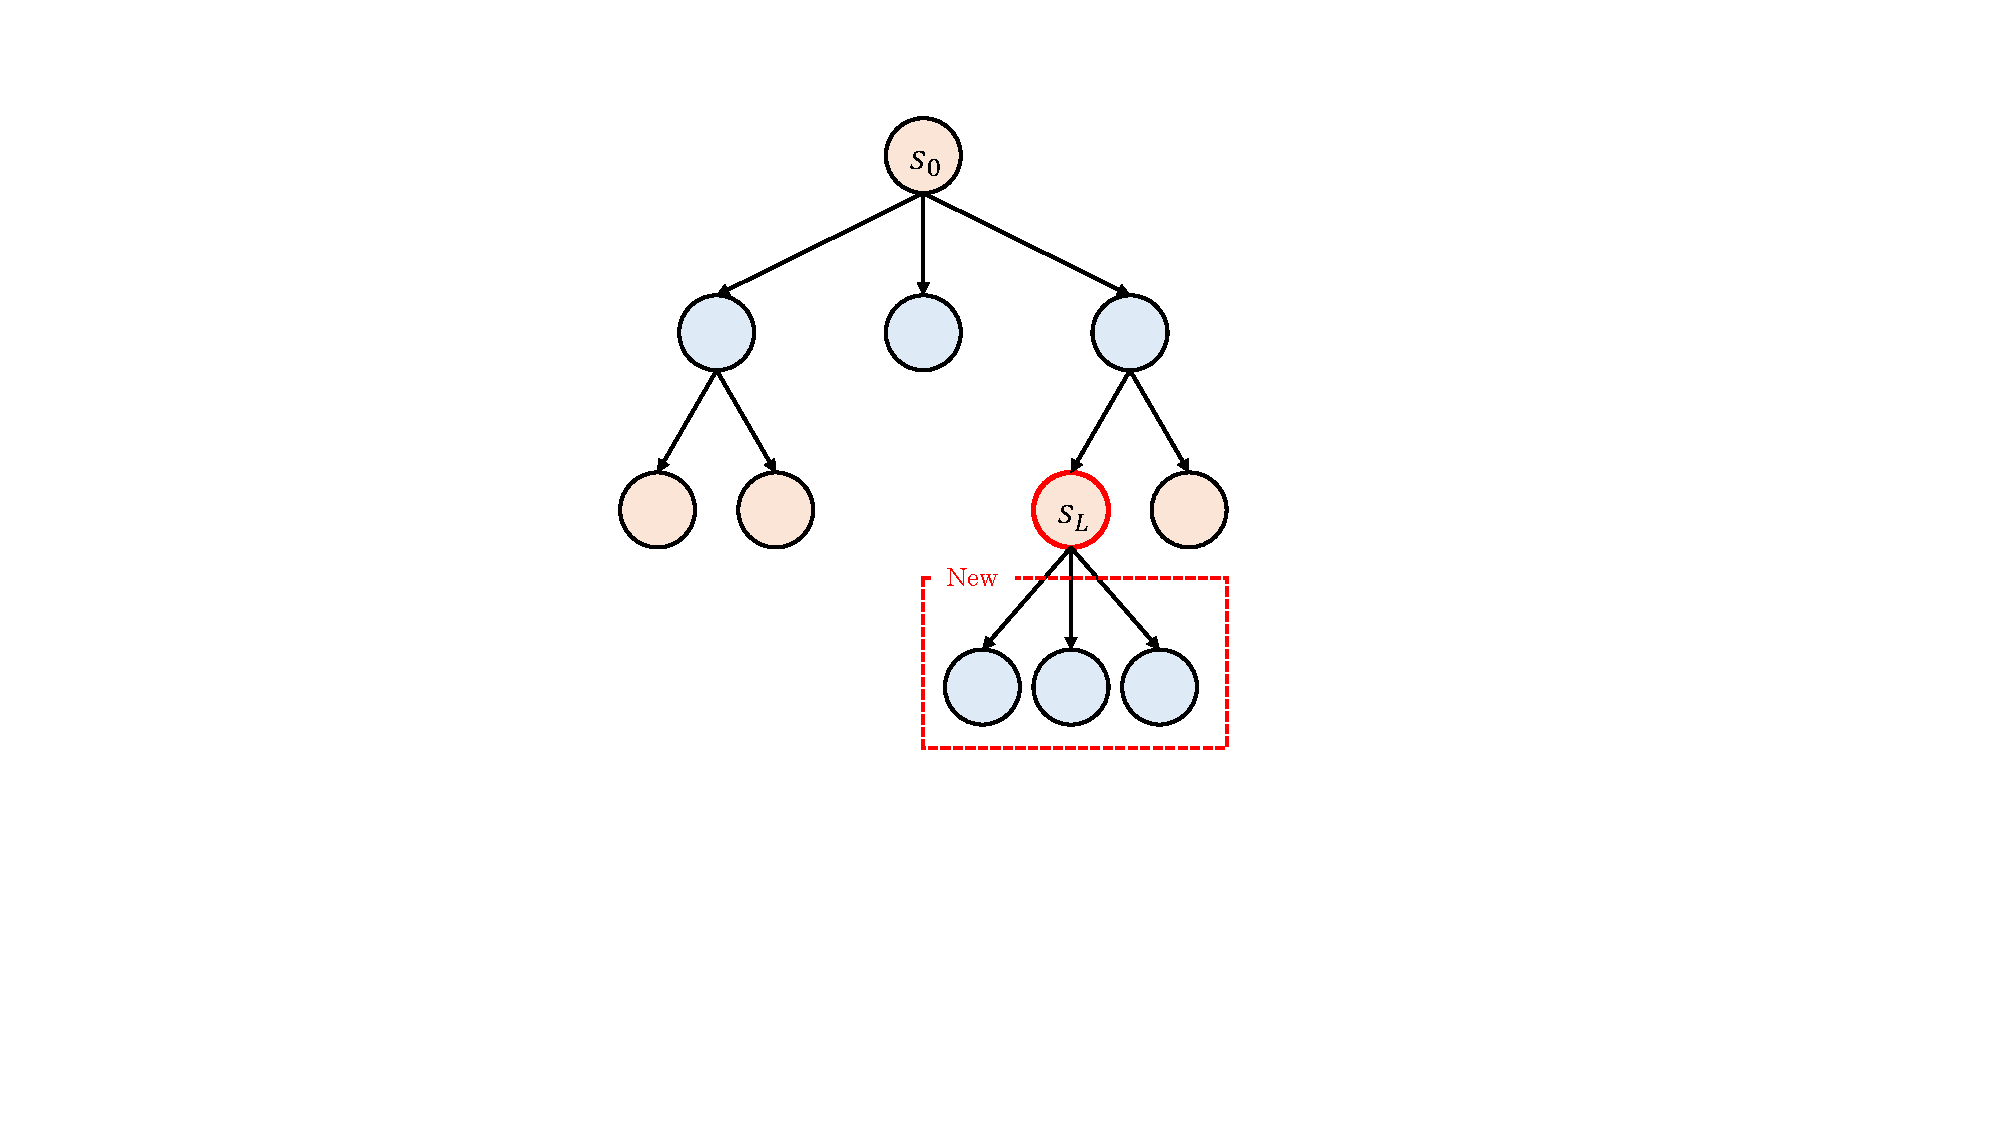
\includegraphics[width=\columnwidth]{figures/expand_.pdf}
    \caption{展開}
    \label{fig:expand}
  \end{subfigure}
  \caption{MCTSの各ステップ~(オレンジ色のノードはdecisionノード, 青色のノードはchanceノード)}
  \label{fig:mcts}
\end{figure}

\subsubsection*{行動の決定方法}
一定回数のシミュレーションを行った後に, 実際に選ぶ行動を決定する.
根ノード$s_0$のそれぞれの子chanceノード$s_c$について, $N(s_c)^{1/\tau}$に比例した確率で子ノードを選択する.
選択した子ノードに対応するafterstateに遷移するような行動をとる.
$\tau$は温度パラメータと呼ばれ, $0$に近づくほど訪問回数に関して貪欲な選択をするようになる.
多様な学習データを集めるために学習の序盤では$\tau$を大きく設定し, 学習が進むについて$0$に近づける.

\subsubsection*{ニューラルネットワークの学習}
MCTSによるプレイによって得たデータを使ってニューラルネットワークを訓練する.
ニューラルネットワークが評価する
各訪問回数を正規化した$\pmb{\pi}$
すなわち式~\ref{eq:az_loss}で表される誤差関数$l$を最小化するようにパラメータを更新する.
\begin{align}
\label{eq:az_loss}
l = (z-v)^2 - \pmb{\pi}^{\mathrm{T}} \log \mathbf{p}
\end{align}
ただし実際の価値関数の学習においては付録~\ref{subsec:nn_impl}節で説明するように, 最小二乗誤差ではなくCross Entropy誤差を最小化するようにパラメータを更新する.


\subsection{先行研究の考察}
\section{2048のミニゲームの完全解析}
\label{chap:solving}
\ref{chap:rl}章で述べた強化学習は環境~(ゲーム)~と何度もやり取りすることで, 最適な方策を学習するための手法である.
一方で小さなゲームであれば, 力ずくの計算によってゲームを完全に解くこともできる.
本章では2048を解析的なアプローチによって解くことについて考察する.

\subsection{2048の完全解析とは}
\label{sec:solving}
2048は$1$人用のゲームであるため, 勝敗のようなプレイヤの明確な目標は存在しない.
そのためプレイヤが何を目標とするかによって, プレイヤの最善手の定義は変化する.
また\ref{sec:rule}節で述べたようにゲームはランダム性を伴うため, 同じ状態から毎回同じ手を選んでも結果は確率的に変動する.

そこで本稿ではある状態$s$における最善手を「$s$から獲得できる得点の合計の期待値が最も高くなるような手」と定義する.
これは~\ref{chap:rl}節で述べた強化学習の最適状態価値と等価なものである.
よって状態$s$から最善手を選び続けて獲得できる得点の合計の期待値を状態$s$の最適価値と呼び, $v_*(s)$で表すことにする.

このとき$v_*(s)$は式~\ref{eq:value}のように再帰的な形式で書くことができる.
\begin{align}
    v_*(s) =
    \begin{cases}
        0 & (s \text{が終了状態}) \\
        \max_a \left(r(s,a) + \mathbb{E}_{s_\text{next} \in \mathcal{T}(s,a)} v_*(s_\text{next}) \right) & (\text{otherwise})
    \end{cases}
    \label{eq:value}
\end{align}
ただし$r(s,a)$は状態$s$から行動$a$をとって獲得する得点, $s_\text{next} \in \mathcal{T}(s,a)$は状態$s$から行動$a$をとって遷移しうる次の状態の集合を表す~(図~\ref{fig:state_afterstate}を参照).
式~\ref{eq:value}の$r(s,a) + \mathbb{E}_{s_\text{next} \in \mathcal{T}(s,a)} v_*(s_\text{next})$は, 強化学習における最適行動価値$q_*(s,a)$に対応する.
また$\mathbb{E}_{s_\text{next} \in \mathcal{T}(s,a)} v_*(s_\text{next})$は, $s$から$a$をとって遷移するafterstate $s'$の価値といえる.

\begin{figure}[t]
    \centering
    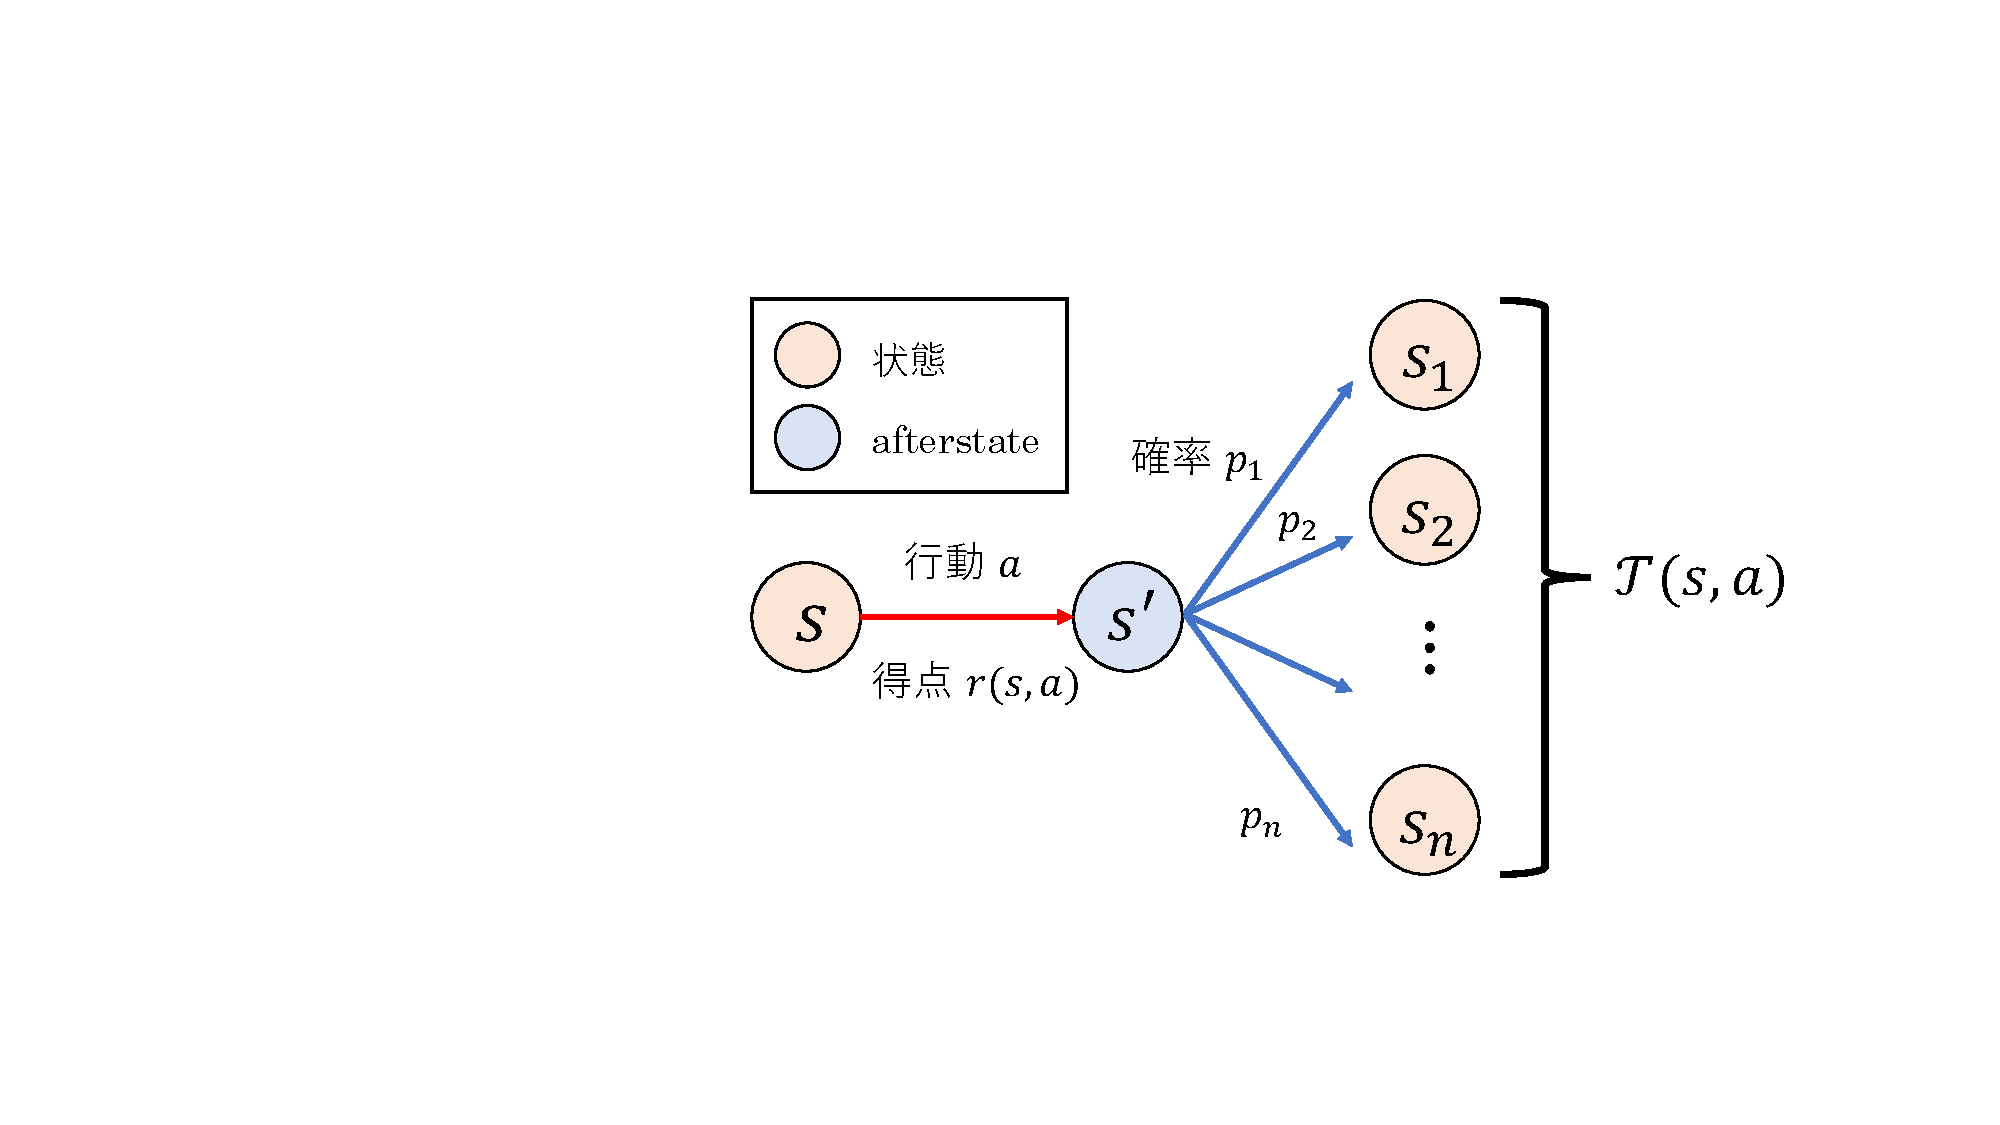
\includegraphics[width=0.6\linewidth{}]{figures/value_function_.pdf}
    \caption{式~\ref{eq:value}の補足図}
    \label{fig:state_afterstate}
\end{figure}

ゲームに現れうるすべての状態の最適価値を計算すれば, 任意の状態において最善手を選ぶことができる.
本稿ではこれを2048の完全解析ということにする.

完全解析をすることで, ゲームの任意の状態の最適価値・最善手を明かし, 最善手を選び続けるプレイヤの戦略を解析することができる.
さらに2048を対象とした強化学習手法の良し悪しを定量的に評価し, より良い手法を提案することができると考えられる.
一方で2048を完全解析することは, そのゲーム木の大きさによる計算コストの観点から現状難しいと考えられる.
そこで本来$4\times4$盤面上で行われる2048のミニゲームとして, 盤面サイズを縮小した2048を完全解析することを考える.

\subsection{盤面サイズが小さな2048の完全解析}
\label{sec:mini2048}
基本的なルールは2048と同じで盤面サイズを$4\times4$から縮小したゲームを完全解析することを考える.
盤面サイズに関わらず, 以下の$2$つのステップを順番に行うことで2048を完全解析することができる.

\begin{enumerate}
    \item ゲームに現れうるすべての状態の列挙
    \item 列挙した状態の価値の計算
\end{enumerate}

\ref{subsec:enumeration}節と~\ref{subsec:calculation}節で具体的な方法について述べる.
なお本節の内容は文献~\cite{3x3_2048}および文献~\cite{4x3_2048}を元に執筆された.

\subsubsection{幅優先探索によるすべての状態の列挙}
\label{subsec:enumeration}
完全解析の第1ステップとして幅優先探索によってゲームに現れうるすべての状態を列挙する.
まず初期状態をキューに詰めて探索を開始する.
キューの先頭の状態$s$を取り出し, $s$から遷移可能な次の状態$s_{\text{next}} \in \mathcal{T}(s)$をキューに追加する.
これをキューが空になるまで繰り返すことで, すべての状態を列挙することができる.

ここで$s_{\text{next}} \in \mathcal{T}(s)$がすでに発見済みであるか確認するために, これまでに発見した状態を管理する集合が必要である.
素朴な方法ではメモリでこれまでに発見した全状態を管理することで行えるが, 状態数が非常に大きな場合にはメモリの容量を超えてしまう.

そこで~\ref{sec:property}節で説明した時刻によってゲーム木を整理する.
時刻$t$の状態は時刻$t+2$か$t+4$の状態にしか遷移しないため, 時刻$t+2$と$t+4$の発見した状態をメモリで管理すれば十分である.
よって時刻が最小の$4$の状態から時刻$2$刻みで順番に列挙を行うことで, ディスクを効率的に活用することができる.
以上を踏まえた疑似コードをAlgorithm~\ref{alg:bfs}に示す.

\begin{algorithm}[tb]
\caption{幅優先探索によるすべての状態の列挙}
\label{alg:bfs}
\begin{algorithmic}[1]
\Function {enumeration}{}
    \For {$t=4$ to $t_{max}$}
        \ForAll {$s_t \in \text{queue}_t$} 
            \ForAll {$s_{t+2} \in \mathcal{T}(s_t)$}
                \State $\text{queue}_{t+2}.\text{push}(s_{t+2})$
            \EndFor
            \ForAll {$s_{t+4} \in \mathcal{T}(s_t)$}
                \State $\text{queue}_{t+4}.\text{push}(s_{t+4})$
            \EndFor
        \EndFor
    \EndFor
\EndFunction
\end{algorithmic}
\end{algorithm}

\subsubsection{後退解析による状態の価値の計算}
\label{subsec:calculation}
\ref{subsec:enumeration}節で列挙した状態の価値を式~\ref{eq:value}に従って計算する.
時刻$t$の状態の価値は, 時刻$t+2$と$t+4$の状態の価値が計算済みであれば計算できる.
よって時刻が最大の状態から順番に走査することで, 効率的にすべての状態の価値を計算できる.
疑似コードをAlgorithm~\ref{alg:calculation}に示す.

\begin{algorithm}[tb]
    \begin{algorithmic}[1]

    \Function {calculation}{$t$}
        \For {$t=t_{max}$ to $4$}
            \State $v(s) = \max_a \left(r(s,a) + \mathbb{E}_{s_\text{next} \in \mathcal{T}(s,a)} v_*(s_\text{next}) \right)$
        \EndFor
        \ForAll {$s_t \in \text{queue}_t$} 
            \ForAll {$s_{t+2} \gets s_t$}
                \State $\text{queue}_{t+2}.\text{push}(s_{t+2})$
            \EndFor
            \If {$element > max$}
                \State $max \gets element$
            \EndIf
        \EndFor
        \State \Return $max$
    \EndFunction
    \end{algorithmic}
    \caption{後退解析による価値計算}
    \label{alg:calculation}
\end{algorithm}

\subsection{実験結果}
$2\times2$盤面から$4\times3$盤面までの2048を完全解析した結果を表~\ref{table: analysis_table}に示す.
\begin{table}[t]
    \centering
    \begin{tabular}{rrr}
        \hline \hline
        盤面サイズ & 状態数 & 初期状態の価値\\ \hline
        $2\times2=4$ & $110$ & $67.6$ \\
        $3\times2=6$ & $21,752$ & $480.9$ \\
        $4\times2=8$ & $4,980,767$ & $2,642.6$ \\
        $3\times3=9$ & $48,713,519$ & $5,469.2$ \\
        $4\times3=12$ & $1,152,817,492,752$ & $50,724.2$ \\
        \hline
    \end{tabular}
    \caption{盤面の大きさと解析結果に関する表}
    \label{table: analysis_table}
\end{table}
盤面サイズが大きくなるに従って指数関数的に状態数は大きくなることが分かる.
また初期状態の価値は, 盤面サイズが$n$マス増える度に$2^n \sim 2^{n+1}$倍になっていることが分かる.
そのため$4\times4$盤面の2048は完全解析を行うには状態数が非常に大きく, 初期状態の価値は約$800,000$点程度ではないかと予想される.

$3\times3$盤面と$4\times3$盤面の2048の各時刻における状態数のグラフを図~\ref{fig:state_afterstate}に示す.
多くのゲームでは進行に従って多様な盤面が存在するため状態数は大きくなり続ける.
一方で2048は盤面が数字タイルで埋まるとゲームオーバーになりやすく, その時刻の状態数は少なくなる.
大きな数字タイルを完成させると盤面上に空きマスが増え, ゲームは再び複雑性を増す.
実際, 図~\ref{fig:state_afterstate}からは$2^n$の前後の時刻で状態数が大きく増減していることが見て取れる.
よって2048はゲームの進行に従って, ゲームの複雑性が増減するという特徴を持つ.
このため任意の時刻における状態数は一定の上限で抑えられ, ~\ref{subsec:enumeration}節と~\ref{subsec:calculation}節で説明した完全解析を実行できる.
\begin{figure}
\vspace{0.2cm}
\begin{subfigure}[T]{0.3\columnwidth}
    \centering
    \includegraphics[width=\columnwidth]{figures/graph_mini_.pdf}
    \caption{$3\times3$盤面の2048}
    \label{fig:graph_mini}
\end{subfigure}
\begin{subfigure}[T]{0.3\columnwidth}
    \centering
    \includegraphics[width=\columnwidth]{figures/graph_mid_.pdf}
    \caption{$4\times3$盤面の2048}
    \label{fig:graph_mid}
\end{subfigure}
\begin{subfigure}[T]{0.3\columnwidth}
    \centering
    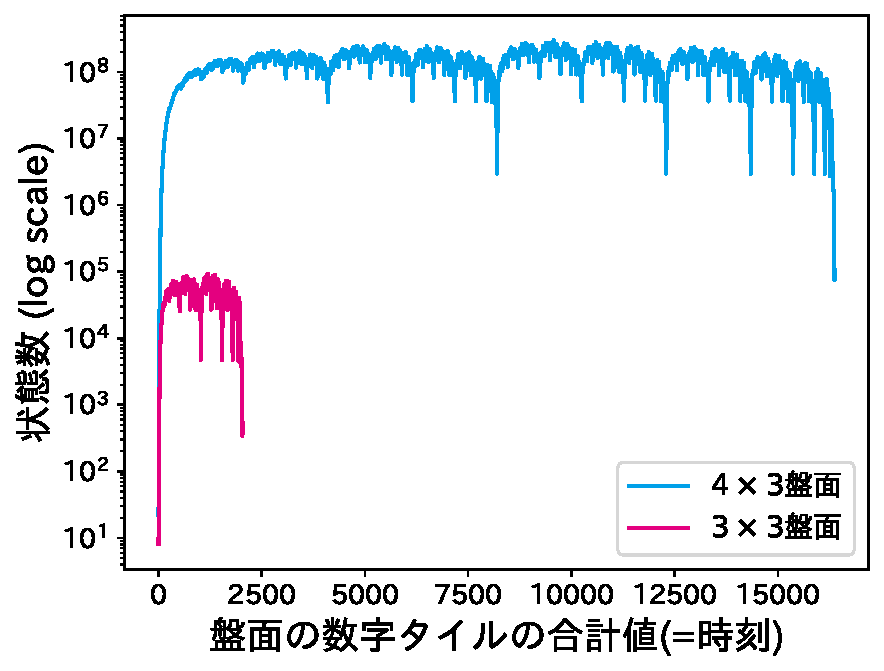
\includegraphics[width=\columnwidth]{figures/graph_compare_mid_mini_.pdf}
    \caption{$3\times3$盤面と$4\times3$盤面の状態数の比較}
    \label{fig:graph_compare_mid_mini_}
\end{subfigure}
\caption{時刻と状態数のグラフ}
\label{fig:time_state_num}
\end{figure}

参考として, $2\times2$盤面の2048のゲーム木全体を図~\ref{fig:game_tree}に示す.
ゲーム木が増大と縮小を繰り返す様子が見て取れる.
\begin{figure}[t]
    \centering
    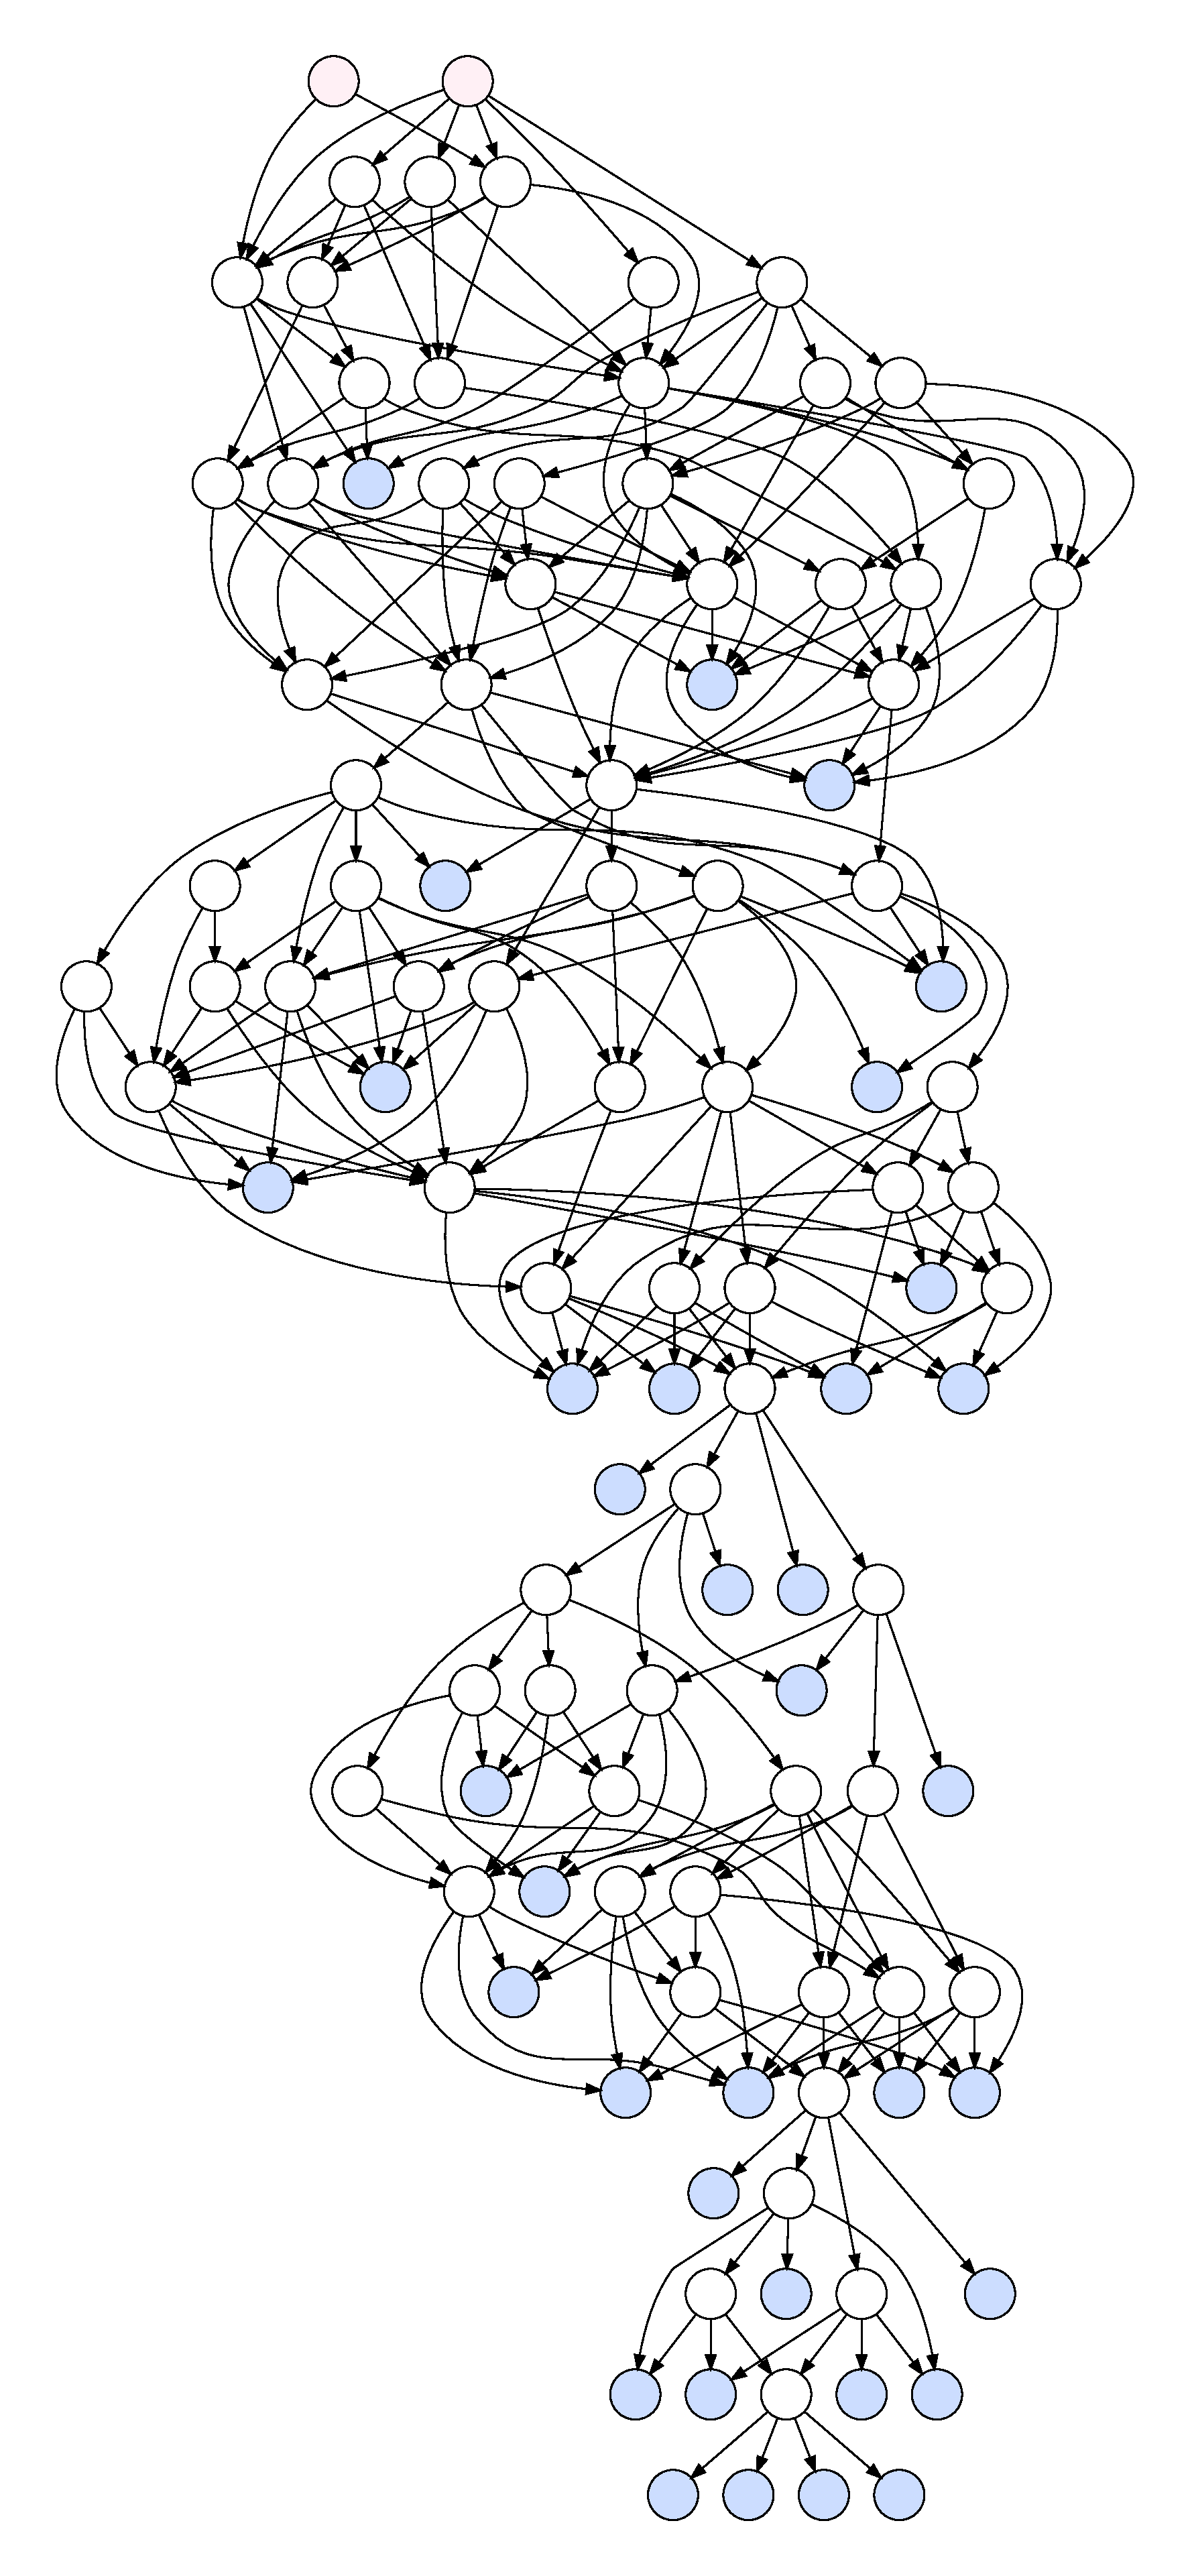
\includegraphics[width=0.7\linewidth{}]{figures/tree.pdf}
    \caption{$2\times2$盤面の2048のゲーム木~(赤色のノードは初期状態, 青色のノードは終了状態)}
    \label{fig:game_tree}
\end{figure}

\appendix
\chapter{実装の詳細}

\section{ゲーム環境の実装}
2048は状態からafterstateへの遷移において, 各行~(列)~の変化は独立に考えることができる.
また回転と反転を考慮することで上下左右は等価な盤面変化を起こす.
よって$1$行の全パターンについて, ある一方向を選択したときの遷移先を前もって計算することで, 全方向に対する盤面全体の遷移を高速に行える.

\section{完全解析の実装}
回転・反転に関して同じ盤面は$1$つの状態として扱った.
またそれぞれの状態は$64$ビット整数で表現された.

$3\times3$盤面の2048の完全解析は状態列挙, 価値計算

\section{強化学習の実装}
\subsection{ニューラルネットワークの詳細}
ニューラルネットワークは盤面の特徴量を入力として, 方策と価値を出力する.
盤面サイズ$H \times W$のルールの下では理論上の最高到達タイルは$2^{H \times W + 1}$である.
このとき入力は空きマス$H \times W + 2$チャネルの$H \times W$から成る.
$n$番目のチャネルの$(i,j)$成分には盤面の$(i,j)$
\begin{figure}[t]
    \centering
    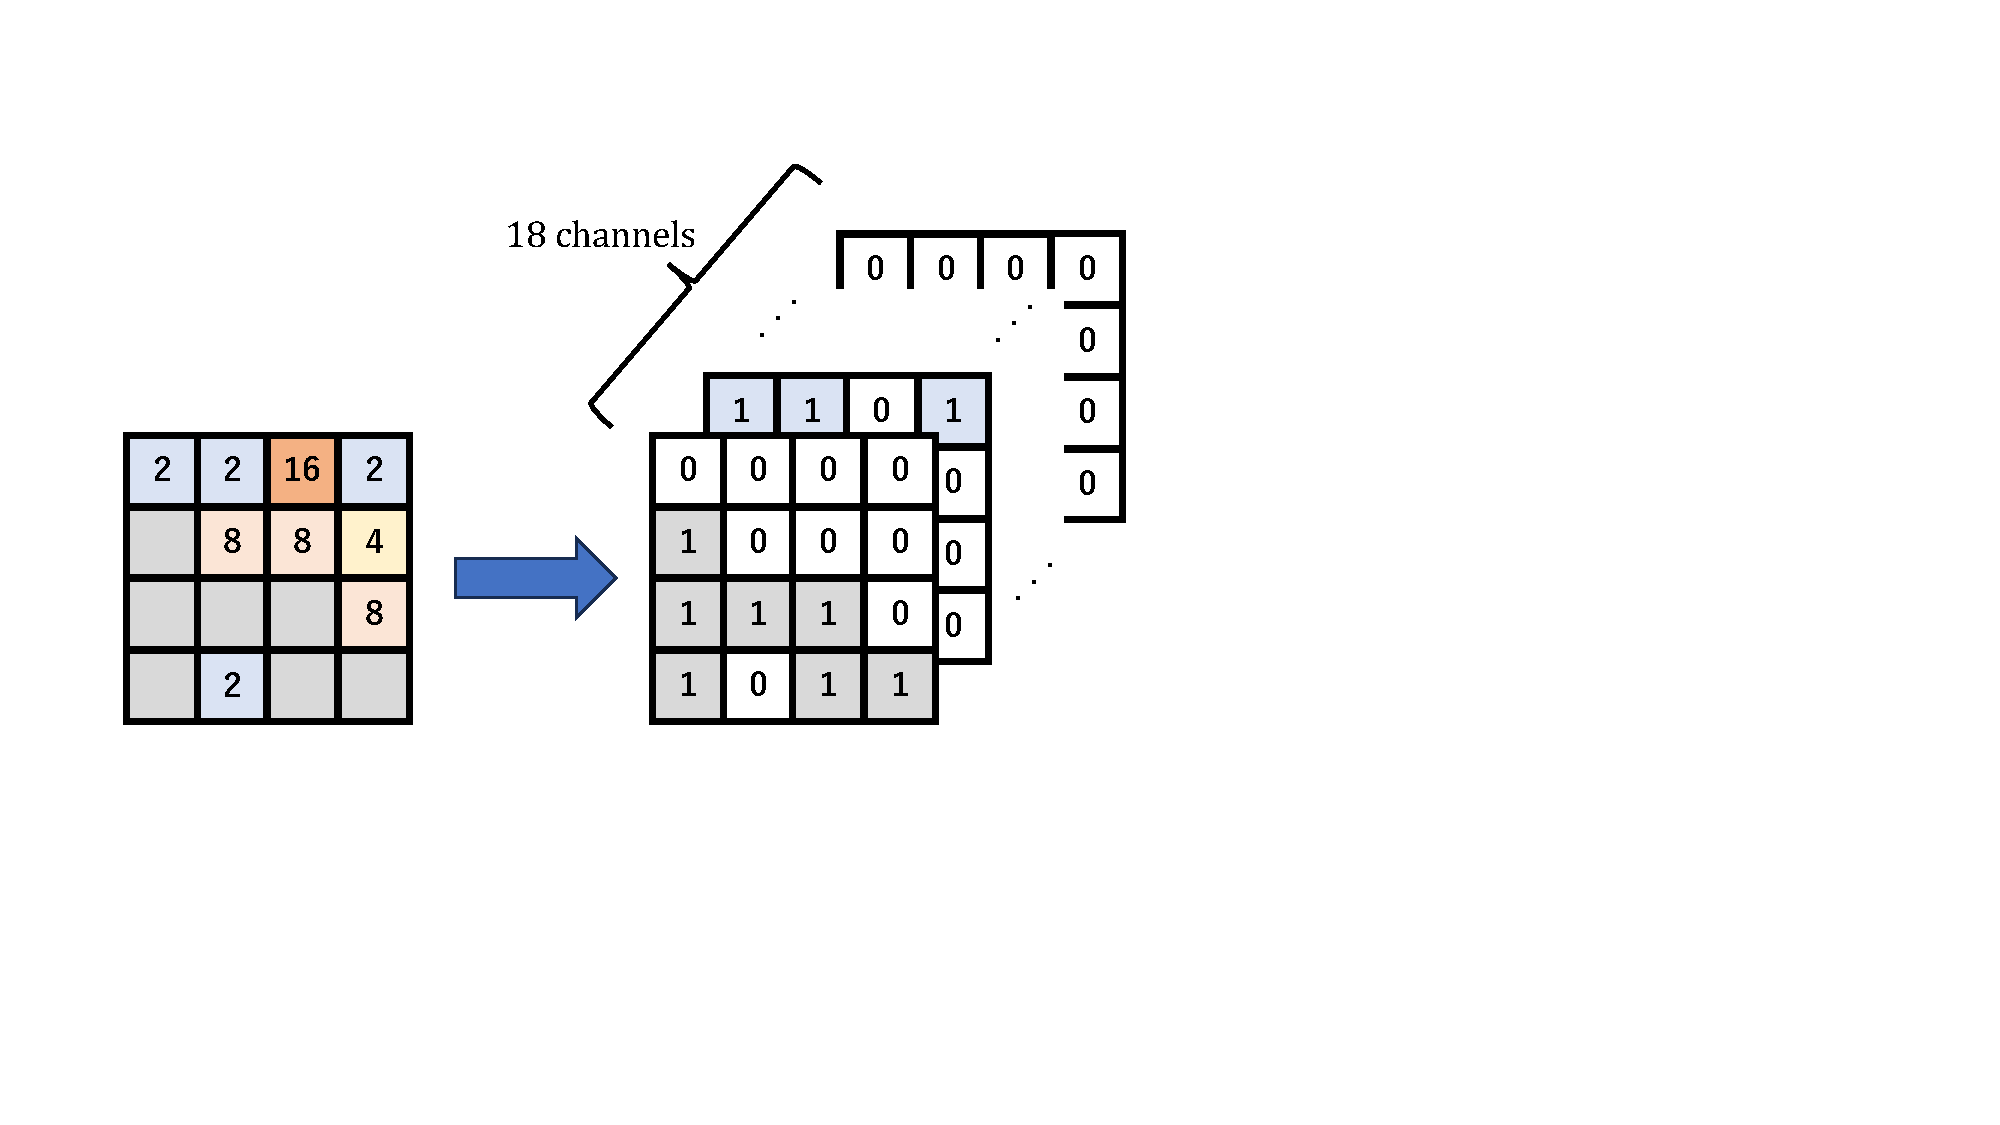
\includegraphics[width=0.6\linewidth{}]{figures/encoding.pdf}
    \caption{ニューラルネットワークへの入力特徴量}
    \label{fig:input_encoding}
\end{figure}

またStochastic MuZero~\cite{StochasticMuZero}に倣って, ニューラルネットワークは価値を$D$次元のベクトル値として出力する.
価値の学習ターゲット$x$~(スカラー値)~は, まず$h(x)= \sqrt{x+1} - 1 + \epsilon x \ (\epsilon=0.001)$によってスケールを調整する~(図~\ref{fig:transform}を参照).
\begin{figure}[t]
    \centering
    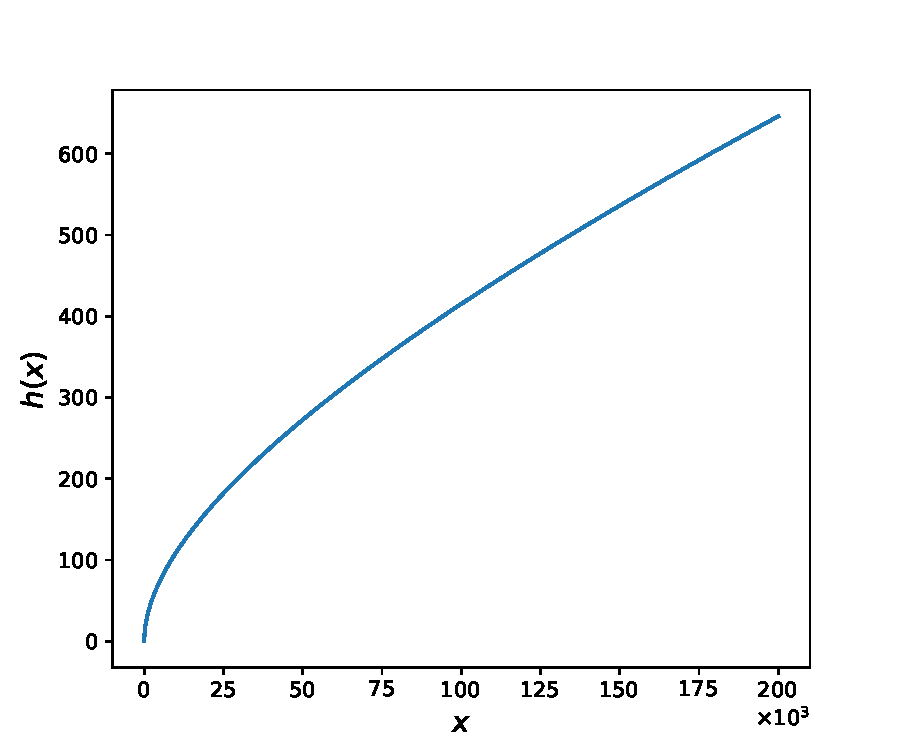
\includegraphics[width=0.6\linewidth{}]{figures/transform_.pdf}
    \caption{$h(x)$のグラフ}
    \label{fig:transform}
\end{figure}
さらに$h(x)$はtwo-hotという, 特定の$2$つの要素以外は全ての$0$であるようなベクトル値に変換される.
たとえば$h(x)=3.7$の場合, $3.7=3 \times 0.3 + 4 \times 0.7$であるため, $3$の重みが$0.3$, $4$の重みが$0.7$, それ以外は$0$である$D$次元ベクトルに変換される.
これをニューラルネットワークの価値の学習ターゲットとして, Cross Entropy誤差を最小化するように訓練される.
推論時にはニューラルネットワークの価値の出力を, softmaxにより全体の総和を$1$にする.
これを$0$から$D$までのそれぞれの重みとして, 重み付け平均$y$を計算する.
最後に$h(x)$の逆関数である$h^{-1}(y)= \epsilon^{-1} (y + 0.5\epsilon^{-1} + 1.0) - 0.5 \sqrt{4.0 \epsilon^{-3} y + 1.004 \epsilon^{-4}}$によって, $x=h^{-1}(y)$を得る.
$3\times3$盤面の2048の実験では$D=200$, $4\times3$盤面では$D=400$, $4\times4$盤面では$D=600$とした.

\subsection{AlphaZeroのニューラルネットワーク}
ニューラルネットワークが出力する価値は, 
ニューラルネットワークは入力に対して方策と価値を出力する.
方策は上下左右それぞれの方向を選択する確率を表す$4$次元のベクトル値である.
価値をベクトル値として出力する.
価値の

\subsection{Prioritized Experience Replayの実装}
Prioritized Experience Replay~\cite{prioritized}は学習に使用するデータを一様ランダムではなく, priorityと呼ばれる重みに従ってサンプルするリプレイバッファである.
リプレイバッファの$i$番目のデータのpriorityを$p_i$とする.
このとき$i$番目のデータはハイパーパラメータ$\alpha$を用いて, 確率$P(i) = \frac{p_{i}^{\alpha}}{\Sigma_k p_{k}^{\alpha}}$でサンプルされる.

Prioritized Experience Replayからのデータのサンプル, およびpriorityの更新は, sum-treeという二分木でデータを管理することで$\mathcal{O}(\log n)$で行うことができる.
sum-treeの葉ノードはpriorityの値を保持し, 各ノードは左右の子ノードの合計値を保持する.
そのため根ノードはpriority全体の合計値$S$を持つ.
サンプルする際には, まず$0$から$S$までの値をランダムに生成し, 根ノードから葉ノードに至るまでたどることで選ぶ.
図~\ref{fig:sumtree}にsum-treeと具体的なサンプルの仕方を例示する.
\begin{figure}[t]
    \centering
    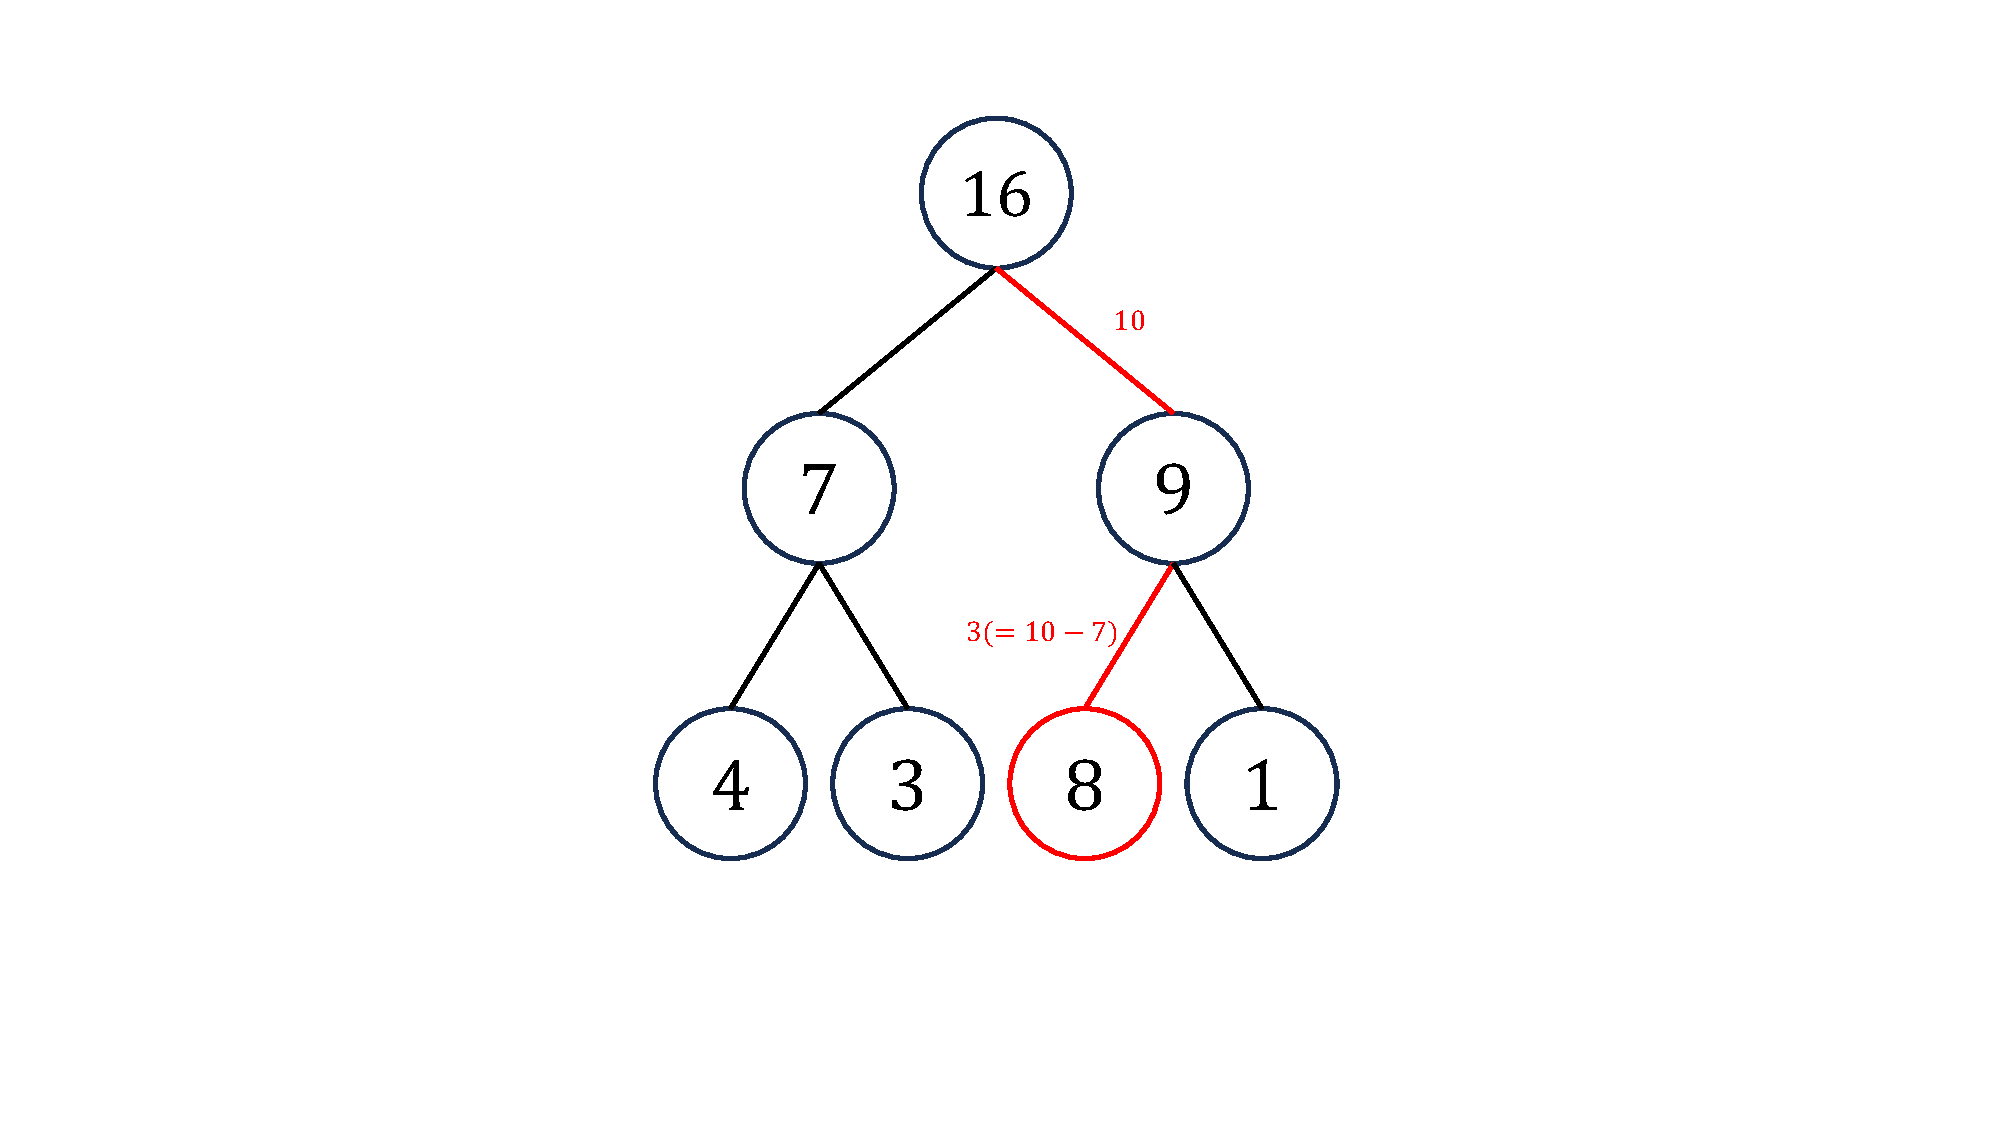
\includegraphics[width=0.4\linewidth{}]{figures/sumtree_.pdf}
    \caption{sum treeの例}
    \label{fig:sumtree}
\end{figure}

\chapter{2048のゲーム性とプレイヤの戦略の検証}
\ref{sec:rule}節で述べたように, 2048の通常のルールではafterstateが次の状態へ遷移する際に出現する, 新しいタイルの数字と位置はランダムに決まる.
すなわちafterstateの空きマスから等確率に選択されたある1マスに$90\%$の確率で$2$のタイルが, $10\%$の確率で$4$のタイルが置かれる.

ここで$2$のタイルと$4$のタイルの出現確率を変更した場合にゲーム性がどう変わるか検証する.
表~\ref{table: value_table}に$3 \times 3$盤面の2048において, $4$の出現確率を通常の$10\%$から増減させたときの完全解析の結果を示す.
表から分かるように, $2$と$4$の出現確率がいずれか一方に傾くほど期待値は大きくなる傾向があることが分かる.
また$4$の出現確率が$0\%$の場合と$100\%$の場合には, 最適な行動をし続ければ常に~図\ref{fig:limit}のような理論上の最終盤面に到達できることが分かる.
2048は$2$と$4$の$2$種類の数字タイルが出現することがゲームを面白くしていると考えられる.
\begin{table}[t]
\caption{4の出現確率を増減させたときのゲームの期待値}
\label{table: value_table}
\centering
\begin{tabular}{r|r||r|r}
    \hline 
    4の確率 & 初期状態の期待値 & 4の確率 & 初期状態の期待値 \\ \hline \hline
    0.00 & 7172.00 & 0.55 & 3206.00 \\
    0.05 & 6161.17 & 0.60 & 3171.24 \\
    \textbf{0.10} & \textbf{5468.49} & 0.65 & 3165.36 \\
    0.15 & 4932.54 & 0.70 & 3194.44 \\
    0.20 & 4515.42 & 0.75 & 3269.18 \\
    0.25 & 4182.44 & 0.80 & 3399.20 \\
    0.30 & 3919.20 & 0.85 & 3607.78 \\
    0.35 & 3704.44 & 0.90 & 3993.30 \\
    0.40 & 3531.46 & 0.95 & 4938.20 \\
    0.45 & 3390.19 & 1.00 & 14344.00 \\
    0.50 & 3278.70 &  & \\
    \hline
\end{tabular}
\end{table}

さらに環境が常にプレイヤにとって最も都合の悪くなるように, 新しい数字タイルを出現させるゲームを考える.
これは得点を最大化したいプレイヤと得点を最小化したい環境の対戦ゲームのように考えることができる.
そのため二人零和有限完全確定情報ゲームと同様に, minmax法によってすべての状態の価値$v_{\text{minmax}}$を計算することができる.
具体的には以下の式~\ref{eq:minmax}に従って, ~\ref{sec:solving}節と同様に後退解析を行えばよい.
環境にランダム性がないため, $v_{\text{minmax}}$は常に固定の値をとる.
\begin{align}
    v_{\text{minmax}}(s) =
    \begin{cases}
        0 & (s \text{が終了状態}) \\
        \max_a \left(r(s,a) + \min_{s_\text{next} \in \mathcal{T}(s,a)} v_{\text{minmax}}(s_\text{next}) \right) & (\text{otherwise})
    \end{cases}
    \label{eq:minmax}
\end{align}

さらに$v_{\text{minmax}}$を評価関数として, 通常のルールでプレイさせることを考える.
悲観的な
よってこれをminmaxプレイヤと呼ぶことにする.
一方で常に都合の良い場合を想定して行動する楽観的な戦略も考えられる.
minmaxプレイヤと対比して, これをmaxmaxプレイヤと呼ぶことにする.

次に

\bibliography{ref} % 研究に役に立ちそうならなんでも入れとく
\bibliographystyle{junsrt}

\end{document}